%File: anonymous-submission-latex-2025.tex
\documentclass[letterpaper]{article} % DO NOT CHANGE THIS
\usepackage[submission]{aaai25}  % DO NOT CHANGE THIS

\usepackage{times}  % DO NOT CHANGE THIS
\usepackage{helvet}  % DO NOT CHANGE THIS
\usepackage{courier}  % DO NOT CHANGE THIS
\usepackage[hyphens]{url}  % DO NOT CHANGE THIS
\usepackage{graphicx} % DO NOT CHANGE THIS
\urlstyle{rm} % DO NOT CHANGE THIS
\def\UrlFont{\rm}  % DO NOT CHANGE THIS
\usepackage{natbib}  % DO NOT CHANGE THIS AND DO NOT ADD ANY OPTIONS TO IT
\usepackage{caption} % DO NOT CHANGE THIS AND DO NOT ADD ANY OPTIONS TO IT
\frenchspacing  % DO NOT CHANGE THIS
\setlength{\pdfpagewidth}{8.5in} % DO NOT CHANGE THIS
\setlength{\pdfpageheight}{11in} % DO NOT CHANGE THIS
%
% These are recommended to typeset algorithms but not required. See the subsubsection on algorithms. Remove them if you don't have algorithms in your paper.
\usepackage{algorithm,algorithmicx}
\usepackage[noend]{algpseudocode}
%
% These are are recommended to typeset listings but not required. See the subsubsection on listing. Remove this block if you don't have listings in your paper.
\usepackage{newfloat}
\usepackage{listings}

\usepackage{subfiles}
\usepackage[utf8]{inputenc} % allow utf-8 input
\usepackage[T1]{fontenc}    % use 8-bit T1 fonts
%\usepackage{hyperref}       % hyperlinks
%\usepackage{url}            % simple URL typesetting
\usepackage{booktabs}       % professional-quality tables
\usepackage{amsfonts}       % blackboard math symbols
\usepackage{nicefrac}       % compact symbols for 1/2, etc.
\usepackage{microtype}      % microtypography
\usepackage{xcolor}         % colors
\usepackage{mathtools}

\usepackage{subcaption}
\usepackage{tabularx}
\usepackage{thmtools, thm-restate}
\usepackage{dsfont}
\usepackage{enumitem}
\usepackage{fontawesome5,xspace}
\usepackage{amsmath,amssymb}
\usepackage{amsthm}
\usepackage{bm}

\newcommand{\TopH}{\texttt{Top2}}
\newcommand{\CMP}{\texttt{CMP}}
\newcommand{\HDETC}{\texttt{HD-ETC}}
\newcommand{\EBHDETC}{\texttt{EBHD-ETC}}
\newcommand{\MLAS}{\texttt{MLAS}}
\newcommand{\KL}{\texttt{kl-UCB}}
\newcommand{\DMP}{\texttt{DMP}}
\newcommand{\CDM}{\texttt{CDM}}
\newcommand{\Phii}{\texttt{PHI}}
\newcommand{\UCB}{\texttt{UCB}}
\newcommand{\HCLA}{\texttt{HCLA}}
\newcommand{\GHCLA}{\texttt{G-HCLA}}
\newcommand{\GPHCLA}{\texttt{GP-HCLA}}
\newcommand{\HALG}{\texttt{Hungarian}}
\newcommand{\D}{\texttt{D}}
\newcommand{\C}{\texttt{C}}

\newcommand{\WHHMMAB}{\texttt{WH$^2$MMAB}}
\newcommand{\SHHMMAB}{\texttt{SH$^2$MMAB}}
\newcommand{\sta}{\texttt{Send2All}}
\newcommand{\rcv}{\texttt{Receive}}
\newcommand{\HMMAB}{\texttt{H$($M$)^2$AB}}
\newcommand{\HDAC}{\texttt{HDAC}}
\newcommand{\allprobe}{\texttt{AllProbe}}
\newcommand{\HHMMAB}{\texttt{HMA2B}}
\newcommand{\ghint}{G^{\text{hint}}}
\DeclareMathOperator*{\argmax}{arg\,max}
\DeclareMathOperator*{\argmin}{arg\,min}


\newcommand{\mo}[1]{{\textcolor{blue}{[MH says: #1]}}}
\newcommand{\rev}[1]{{\textcolor{red}{#1}}}

\newtheorem{theorem}{Theorem}
\newtheorem{lemma}{Lemma}
\newtheorem{observation}{Observation}


\newcommand{\GS}{\texttt{Gale-Shapley}}
\newcommand{\bb}[1]{\mathbb{#1}}


\newcommand{\xw}[1]{\todo{XW: #1}}
\newcommand{\am}[1]{{\textcolor{red}{Amirmahdi: #1}}}

\newtheorem{corollary}{Corollary}

\newtheorem{definition}{Definition}


\usepackage{array}
\newcolumntype{P}[1]{>{\centering\arraybackslash}p{#1}}


\DeclareMathOperator{\E}{\mathbb{E}}
\DeclarePairedDelimiter{\ceil}{\lceil}{\rceil}

\newcommand{\1}[1]{\mathds{1}{\{#1\}}}

\renewcommand{\check}{{\textcolor{green}{\faCheck}\xspace}}
\newcommand{\question}{{\textcolor{blue}{\faQuestion}\xspace}}
\newcommand{\xtimes}{{\textcolor{blue}{\faTimes}\xspace}}
\newcommand{\todocircle}{{\textcolor{blue}{\faCircle[regular]}\xspace}}
\newcommand{\abs}[1]{\left\lvert#1\right\rvert}
\usepackage[colorinlistoftodos,prependcaption,textsize=tiny,textwidth=1cm,color=green]{todonotes}

\let\oldComment=\Comment
\renewcommand{\Comment}[1]{\oldComment{\texttt{#1}}}
\algnewcommand{\LeftComment}[1]{\Statex $\triangleright$ \texttt{#1}}
\algnewcommand{\RightComment}[1]{\Statex \leavevmode\hfill$\triangleright$ \texttt{#1}}

\algnewcommand\algorithmicinput{\textbf{Input:}}
\algnewcommand\Input{\item[\algorithmicinput]}%

\algnewcommand\algorithmicoutput{\textbf{Output:}}
\algnewcommand\Output{\item[\algorithmicoutput]}%

\algnewcommand\algorithmicinitial{\textbf{Initialize:}}
\algnewcommand\Initial{\item[\algorithmicinitial]}%

\DeclareCaptionStyle{ruled}{labelfont=normalfont,labelsep=colon,strut=off} % DO NOT CHANGE THIS
\lstset{%
	basicstyle={\footnotesize\ttfamily},% footnotesize acceptable for monospace
	numbers=left,numberstyle=\footnotesize,xleftmargin=2em,% show line numbers, remove this entire line if you don't want the numbers.
	aboveskip=0pt,belowskip=0pt,%
	showstringspaces=false,tabsize=2,breaklines=true}
\floatstyle{ruled}
\newfloat{listing}{tb}{lst}{}
\floatname{listing}{Listing}
%
% Keep the \pdfinfo as shown here. There's no need
% for you to add the /Title and /Author tags.
\pdfinfo{
/TemplateVersion (2025.1)
}


% DISALLOWED PACKAGES
% \usepackage{authblk} -- This package is specifically forbidden
% \usepackage{balance} -- This package is specifically forbidden
% \usepackage{color (if used in text)
% \usepackage{CJK} -- This package is specifically forbidden
% \usepackage{float} -- This package is specifically forbidden
% \usepackage{flushend} -- This package is specifically forbidden
% \usepackage{fontenc} -- This package is specifically forbidden
% \usepackage{fullpage} -- This package is specifically forbidden
% \usepackage{geometry} -- This package is specifically forbidden
% \usepackage{grffile} -- This package is specifically forbidden
% \usepackage{hyperref} -- This package is specifically forbidden
% \usepackage{navigator} -- This package is specifically forbidden
% (or any other package that embeds links such as navigator or hyperref)
% \indentfirst} -- This package is specifically forbidden
% \layout} -- This package is specifically forbidden
% \multicol} -- This package is specifically forbidden
% \nameref} -- This package is specifically forbidden
% \usepackage{savetrees} -- This package is specifically forbidden
% \usepackage{setspace} -- This package is specifically forbidden
% \usepackage{stfloats} -- This package is specifically forbidden
% \usepackage{tabu} -- This package is specifically forbidden
% \usepackage{titlesec} -- This package is specifically forbidden
% \usepackage{tocbibind} -- This package is specifically forbidden
% \usepackage{ulem} -- This package is specifically forbidden
% \usepackage{wrapfig} -- This package is specifically forbidden
% DISALLOWED COMMANDS
% \nocopyright -- Your paper will not be published if you use this command
% \addtolength -- This command may not be used
% \balance -- This command may not be used
% \baselinestretch -- Your paper will not be published if you use this command
% \clearpage -- No page breaks of any kind may be used for the final version of your paper
% \columnsep -- This command may not be used
% \newpage -- No page breaks of any kind may be used for the final version of your paper
% \pagebreak -- No page breaks of any kind may be used for the final version of your paperr
% \pagestyle -- This command may not be used
% \tiny -- This is not an acceptable font size.
% \vspace{- -- No negative value may be used in proximity of a caption, figure, table, section, subsection, subsubsection, or reference
% \vskip{- -- No negative value may be used to alter spacing above or below a caption, figure, table, section, subsection, subsubsection, or reference

\setcounter{secnumdepth}{2} %May be changed to 1 or 2 if section numbers are desired.

% The file aaai25.sty is the style file for AAAI Press
% proceedings, working notes, and technical reports.
%

% Title

% Your title must be in mixed case, not sentence case.
% That means all verbs (including short verbs like be, is, using,and go),
% nouns, adverbs, adjectives should be capitalized, including both words in hyphenated terms, while
% articles, conjunctions, and prepositions are lower case unless they
% directly follow a colon or long dash
\title{Heterogeneous Multi-Agent Bandits
    with Parsimonious Hints}
\author{
    %Authors
    % All authors must be in the same font size and format.
    Written by AAAI Press Staff\textsuperscript{\rm 1}\thanks{With help from the AAAI Publications Committee.}\\
    AAAI Style Contributions by Pater Patel Schneider,
    Sunil Issar,\\
    J. Scott Penberthy,
    George Ferguson,
    Hans Guesgen,
    Francisco Cruz\equalcontrib,
    Marc Pujol-Gonzalez\equalcontrib
}
\affiliations{
    %Afiliations
    \textsuperscript{\rm 1}Association for the Advancement of Artificial Intelligence\\
    % If you have multiple authors and multiple affiliations
    % use superscripts in text and roman font to identify them.
    % For example,

    % Sunil Issar\textsuperscript{\rm 2},
    % J. Scott Penberthy\textsuperscript{\rm 3},
    % George Ferguson\textsuperscript{\rm 4},
    % Hans Guesgen\textsuperscript{\rm 5}
    % Note that the comma should be placed after the superscript

    1101 Pennsylvania Ave, NW Suite 300\\
    Washington, DC 20004 USA\\
    % email address must be in roman text type, not monospace or sans serif
    proceedings-questions@aaai.org
%
% See more examples next
}

%Example, Single Author, ->> remove \iffalse,\fi and place them surrounding AAAI title to use it
\iffalse
\title{My Publication Title --- Single Author}
\author {
    Author Name
}
\affiliations{
    Affiliation\\
    Affiliation Line 2\\
    name@example.com
}
\fi

\iffalse
%Example, Multiple Authors, ->> remove \iffalse,\fi and place them surrounding AAAI title to use it
\title{My Publication Title --- Multiple Authors}
\author {
    % Authors
    First Author Name\textsuperscript{\rm 1},
    Second Author Name\textsuperscript{\rm 2},
    Third Author Name\textsuperscript{\rm 1}
}
\affiliations {
    % Affiliations
    \textsuperscript{\rm 1}Affiliation 1\\
    \textsuperscript{\rm 2}Affiliation 2\\
    firstAuthor@affiliation1.com, secondAuthor@affilation2.com, thirdAuthor@affiliation1.com
}
\fi


% REMOVE THIS: bibentry
% This is only needed to show inline citations in the guidelines document. You should not need it and can safely delete it.
\usepackage{bibentry}
% END REMOVE bibentry

\begin{document}

\maketitle

\begin{abstract}
We explore hinted heterogeneous multi-agent multi-armed bandits (\texttt{HMA2B}), where agents can query low-cost observations, called hints, in addition to pulling arms. In the \texttt{HMA2B} framework, each of the $M$ agents maintains an individual heterogeneous reward distribution over a fixed set of $K$ arms and can observe the reward of the arm they pull only if no other agent pulls that arm through $T$ rounds of decision making. 

We aim to find a matching with maximum utility by querying the minimum possible hints from the arms without pulling them, thus achieving time-independent regret.
We study \texttt{HMA2B} under both centralized and decentralized setups. In the proposed centralized algorithms \texttt{HCLA} and \texttt{GP-HCLA}, a central decision maker determines which arms each agent should pull or query hints from, achieving $O(M^4K)$ regret with $O(MK\log T)$ queried hints. In contrast, in the decentralized setup, we introduce \texttt{HD-ETC} and \texttt{EBHD-ETC}, where agents independently decide their actions through collision-based communications, achieving $O(M^3K^2)$ regret with $\Theta(M^3K \log T)$ queried hints. Both \texttt{HD-ETC} and \texttt{EBHD-ETC} use uniform hinting for arms but differ in stopping criteria: \texttt{HD-ETC} stops hinting at a fixed time step based on the assumed minimum gap $\Delta_{\min}$, while \texttt{EBHD-ETC} employs an elimination-based approach without knowing the minimum gap. This allows for adaptive hinting and efficient matching in decentralized settings. 
We also prove the necessary asymptotic lower bounds for the number of required hints and communication phases, thereby demonstrating the asymptotic optimality of our results. Lastly, we perform numerical simulations to empirically verify the performance of our proposed algorithms.
 
\end{abstract}


% !TeX root = ../main.tex
% \begin{itemize}
%     \item[\todocircle] Can we prove a lower bound for the number of necessary hints? For the lower bound, it depends on the conditions. One cannot formally state that the bounds are optimal. 
%     \item[\todocircle] Other hint models, e.g., give the confidence interval feedback
%     \item[\todocircle] Compare the literature with predictions in the related works. e.g., literature on expert problems. Check multi-agent experts with heterogeneous rewards.
%     \item[\todocircle] Check whether we need to compare with this work: Balkanski, Eric, et al. "Online mechanism design with predictions." arXiv preprint arXiv:2310.02879 (2023).
% \end{itemize}


\section{Introduction}


Online decision making under uncertainty is a crucial challenge in machine learning, with significant implications for real-world applications such as online resource allocation and labor market employment. In these scenarios, resources like items, radio channels, or job positions must be matched to agents to optimize objectives like throughput, utility, or revenue. Since agents often have different abilities or utilities, the decision maker must make careful matchings. However, accurately determining these abilities or utilities is often impossible, forcing the decision maker to rely on potentially imprecise estimates from exploration and adjustments over time. Imprecise estimations can lead to costly mistakes, such as financial or human resource losses. To mitigate this, low-cost hints related to each possible matching can offer valuable insights into potential utility without requiring costly exploration.  We study such problems and propose online decision-making algorithms that leverage the power of low-cost hints to significantly reduce exploration loss while minimizing the number of queried hints.

We use \emph{Hinted Heterogeneous Multi-Armed Bandits} ($\HHMMAB$), an extension of the \emph{Multi-Armed Bandits} framework \cite{bubeck2012regret,lai1985asymptotically}, to solve problems where multiple agents, each with different preferences, must make decisions. The main challenge is to achieve time-independent regret while using as few hints as possible. This requires identifying sub-optimal matchings that might be overlooked due to the inherent uncertainty in online decision-making. An algorithm must separate exploration and exploitation, making effective use of low-cost hints. The uniform hint inquiry approach, which is similar to the \emph{explore-then-commit} strategy, attempts to do this, but proving its time-independent regret is not straightforward. To improve this, we propose a centralized algorithm, $\GPHCLA$, which performs better in terms of time-independent regret and hint complexity while utilizing the uniform hint inquiry approach for decentralized setups. 

For decentralized settings, we explore a method where agents combine uniform hinting with collision-based communication, which we show is necessary to achieve time-independent regret. The centralized method in $\GPHCLA$ doesn't work well in decentralized setups because it relies on a time-dependent metric $\KL$, which individual agents can't use effectively without knowing the statistics of other agents during exploration phases. Our decentralized algorithms, $\HDETC$ and $\EBHDETC$, face an additional challenge beyond the complex analysis required to prove time-independent regret: the inaccurate statistics that agents gather through communication, caused by sharing decimal statistics using an integral communication protocol.




\subsection{Our Contributions}
We analyze the $\HHMMAB$ problem in both \emph{centralized} and \emph{decentralized} setups. In the centralized setup, an omniscient decision maker determines which matching to pull and which to query for a hint, similar to decision-making in hiring processes where the employer has access to the applicants' information to decide which of them to interview and which to hire. We introduce two algorithms: $\HCLA$ and $\GPHCLA$. Both algorithms compare the empirical mean of the selected matching with the maximum $\KL$ divergence of other matchings, querying for a hint if the divergence exceeds a certain threshold. As shown in Table \ref{demo-table}, both $\GPHCLA$ and $\GHCLA$, which are extensions of $\HCLA$, achieve time-independent regret using an asymptotically optimal number of hints. We also prove that the upper bound we established for the hint complexity of $\GPHCLA$ is tight.

In the decentralized setup, commonly used in radio channel allocation to stations, we propose two algorithms, $\HDETC$ and $\EBHDETC$, which divide the time horizon into \emph{exploration} and \emph{communication} phases. In both algorithms, agents continue querying for hints until they reach a specific time step. The key difference between them is that in $\HDETC$, agents are assumed to know the minimum gap $\Delta^\text{G}_{\min}$ and the time horizon $T$, allowing them to stop hinting at a pre-fixed time step $t'$. In contrast, $\EBHDETC$ uses an edge elimination approach to determine when to stop hinting, making the stopping point a random variable rather than the fixed time step $t'$, which results in slightly more hint queries and regret. We present guaranteed bounds for these algorithms, accounting for the added uncertainty caused by communication.





\begin{table*}[t]
\centering    
\caption{Regret, Queried Hints, and Communication Bounds for Centralized and Decentralized Algorithms}
\label{demo-table}
\begin{tabularx}{1.00\textwidth}{ccccccc}

\toprule
Algorithm &  D/C & Regret & Queried Hints & Communication& Minimum Gap $\Delta^\text{G}_{\min}$& Time Horizon $T$\\
\toprule
$\GHCLA$ \ref{lemma:hcla2}  & C&  $O\left(M^4K\right)$&$O\left(M^2K \log T\right)$&N/A&Unknown&Unknown\\

\midrule
$\GPHCLA$ \ref{routin:hcla1}     & C& $O\left(M^4K\right)$&$O\left(MK \log T\right)$&N/A&Unknown&Unknown\\
\midrule
$\HDETC$ \ref{routin:hdetc} & D&$O\left(M^3K^2\right)$&$\Theta\left(M^3K \log MT\right)$&$\Theta\left(\log T\right)$&Known&Known\\
 \midrule
 $\EBHDETC$ \ref{routin:ebhdetc}  & D&$O\left(M^3K^2\right)$&$\Theta\left(M^3K \log T\sqrt{M}\right)$&$\Theta\left(\log T\right)$&Unknown&Known\\
\bottomrule
\end{tabularx}
\end{table*}

\subsection{Related Works}

\paragraph{Heterogeneous MMAB (HMMAB)} 
HMMAB is one of the standard models in multi-player multi-armed bandits with collision literature, to name a few~\citet{rosenski2016multi,boursier2019sic,mehrabian2020practical,bistritz2018distributed,shi2021heterogeneous}.
Among them, \citet{bistritz2018distributed} was the first to study the HMMAB, where they proposed a decentralized algorithm with $O(\log^2 T)$ regrets.
Later on, the regret bound of this model was improved to \(O(M^3K\log T)\) by~\citet{mehrabian2020practical} and further to \(O(M^2K\log T)\) by~\citet{shi2021heterogeneous} that is the state-of-the-art result.
We are the first to introduce the hint mechanism to HMMAB.


\paragraph{Bandits with Hints} 
Learning algorithm with hints (or predictions) belongs to the emerging learning-augmented literature, e.g.,~\citep{lykouris2021competitive,purohit2018improving,mitzenmacher2022algorithms} etc.
The hint mechanism was first studied in the basic stochastic multi-armed bandits model by~\citet{yun2018multi}, and later, \citet{lindstaahl2020predictive} considers a more realistic hint mechanism (with failure noise) for the same model. Besides this line of work, \citep{bhaskara2023bandit} studied the impact of hints in adversarial bandits recently. 
We are the first to study the hint mechanism in the multi-agent scenario.


\subsection{Hinted Heterogeneous Multi-Agent Multi-Armed Bandits}
\paragraph{Basic model} A Hinted Heterogeneous Multi-agent Multi-Armed Bandit (\texttt{HMA2B}) model consists of a set of $K$ \emph{arms}  \(\mathcal{K}\)  and a set of $M$ \emph{agents} \(\mathcal{M}\), such that \(M < K\).
Agents have heterogeneous \emph{rewards} for arms. That is, for each agent \(m\in \mathcal{M}\), each arm \(k\in\mathcal{K}\) is associated with a Bernoulli reward random variable \(X_{m,k}\) with mean \(\mu_{m,k} \coloneqq \mathbb{E}[X_{m,k}]\).
% This implies that several agents are involved in the same bandit problem, with a real-valued parameter $\mu_{m,k} \in (0,1)$ for each $m \in \mathcal{M}$ and $k \in \mathcal{K}$. 
The heterogeneous reward means are represented by a matrix $\bm{\mu} \in [0,1]^{M\times K}$, where each of its rows is denoted by $\bm{\mu}_m = (\mu_{m,k})_{k\in\mathcal{K}}\in [0,1]^{K}$. 
% When player \(m\in\mathcal{M}\) pulls arm \(k\in\mathcal{K}\), it receives a reward $r_{m}$ sampled from the Bernoulli distribution \(\mathcal{D}_{m,k}\) with \(\mu_{m,k}\) as its mean. 
% where the reward value lies in the interval \([0,1]\)\todo{as KL-UCB is applied, please assume Bernoulli reward directly}. 

% We also will use another notation \(G_m^{-1}\), which returns the only arm that agent $m$ is connected to, $k_m$, in graph \(G\)\todo{\(G_m^{-1}\) and \(k_m\) are the same notation, why not use some notation like \(k_m^{G}\) instead?}. 
\paragraph{Reward feedback} Suppose that \(T\in\mathbb{N}^+\) denotes the total number of decision rounds. At each \emph{time step} \(t\in \{1,2,\dots, T\}\), every agent \(m\) chooses an arm \(k_{m}(t)\) to pull. So, the arms requested by the agents forms a bipartite graph characterized by \(M\) nodes (agents) on one side and \(K\) nodes (arms) on the other comprising \(M\) edges, ensuring that each node on the agent side is connected to exactly one arm.
Let us define \(\mathcal{G}\) as the set of all such graphs. Denote \(G(t) \coloneqq (m, k_m(t))_{m\in\mathcal{M}}\) as the bipartite graph representing the arm pulling graph of the agents at time step \(t\).
We consider the \emph{collision} setting~\citep{boursier2019sic,shi2021heterogeneous}: that is, if there exist other agents pulling the arm \(k_m(t)\) at time step \(t\), then agent \(m\) gets a reward of zero; otherwise, agent \(m\) gets a reward \(X_{m,k_m(t)}(t)\) sampled from the reward distribution of arm \(k_m(t)\), or formally, \(r_m(t) \coloneqq X_{m,k_m(t)}(t)\1{\not\exists m'\neq m: k_{m'}(t) = k_m(t)}\).


Given a matching $G\in\mathcal{G}$ and a reward mean matrix $\bm{\mu} \in [0,1]^{M\times K}$, we define the expected utility of this matching as follows,
{
\footnotesize 

\begin{align*}
 U(G;\bm{\mu}) &\coloneqq \mathbb{E}\left[\sum_{m \in \mathcal{M}}r_{m}\right],\\ &= \sum_{m\in\mathcal{M}} \mu_{m,k_m^G} \1{\not\exists m'\neq m: k_{m'}^G = k_m^G},   
\end{align*}
}

where the \(k_m^G\) denotes the matched arm of agent \(m\) under matching \(G\).
We denote the matching with the highest utility as the optimal matching as 
\(G^* \coloneqq \max_{G \in \mathcal{G}} U(G;\bm{\mu}).\) We assume that $G^*$ is \emph{unique}, i.e., there does not exist any $G\neq G^*$ in $\mathcal{G}$ such that $ U(G;\bm{\mu}) = U(G^*;\bm{\mu})$.
 

\paragraph{Hint mechanism} At each time slot \(t\), besides the pulled arm \(k_m(t)\), agent \(m\) can query another arm \(k_m^{\text{hint}}(t)\) and observe the arm's reward realization \(X_{m,k_m^{\text{hint}}(t)}(t)\) without regret cost. The hint graph then is denoted by $G^{\text{hint}}(t)$ and $k^{G^{\text{hint}}(t)}_m$ is the arm agent $m$ queried a hint for in it. These hint observations do not impact the accumulative reward and regret, and the agent can decide whether to query for a hint, denoted by the indicator function \(\ell^\pi_m(t) \coloneqq \1{\text{agent }m\text{ query a hint at }t\text{ under policy }\pi}\).
We denote \(L^\pi(T) \coloneqq \E\left[\sum_{m\in\mathcal{M}}\sum_{t=1}^T \ell^\pi_m(t)\right]\) as the total number of times of agents querying hints in the \(T\) rounds, and we want to design a learning policy $\pi$ minimizes the \(L^\pi(T)\). 
% \mo{Is hint collision free? clarify that.}

\paragraph{Regret.} We want to find a policy $\pi$ that maximizes the cumulative reward of all agents in the \(T\) decision rounds. 
To evaluate the performance of $\pi$, we define the \emph{regret} of a policy as the difference between the total reward of all agents under the optimal matching \(G^*\) in all decision rounds and the total reward of all agents following the policy \(\pi\), as follows, 
\begin{align}
    R^{\pi}(T) \coloneqq TU(G^*;\bm{\mu}) - \mathbb{E}\left[\sum_{t=1}^{T} U(G(t);\bm \mu )\right],
\end{align}
where the expectation is taken over the randomness of the policy \(\pi\).



Finally, we define the important parameter, minimum gap, which is crucial and appears in the regret bounds of all the following policies we will analyze. According to the definition of regret, all the policies in this work consider each $G \in \mathcal{G}$ as a ``super arm''; thus, the \emph{minimum gap} here should represent the minimum difference between the utility of any matching $G$ and $G^*$. Finally, we define the minimum gap as $\Delta^G_{\min} \coloneqq \min_{G \neq G^* \in \mathcal{G}} U(G^*;\bm{\mu}) - U(G;\bm{\mu})$, which will appear in the results in the following sections as a crucial parameter.

\paragraph{Main Goal and Motivating Example}
Our goal is to design learning policies that leverage the power of hints to reduce the logarithmically large regret bounds established in previous works \cite{shi2021heterogeneous,mehrabian2020practical,wang2020optimal,boursier2019sic} to a preferably time-independent regret, while minimizing the number of hints queried.

We assume that hints are samples from the same distributions as the rewards obtained from pulling arms. Our algorithms use these hints strategically by querying them only when exploring a sub-optimal matching is necessary during committing to the optimal matching. This approach helps avoid the high costs of direct exploration and improves performance by separating the exploration of sub-optimal matchings from the exploitation of the optimal one. This method also allows for the consideration of more complex hint models.


In practical scenarios, where hints are significantly cheaper than direct actions, our approach proves valuable. For example, in labor markets, a well-designed and low-cost interview process can provide insights into candidate suitability without the high costs associated with hiring mistakes. Similarly, in communication networks, using test signals to estimate bandwidth needs can prevent allocating large channels to low-demand stations, thus avoiding disruptions in critical systems like flight control. These applications highlight how our hint-based approach can enhance decision-making and efficiency in various real-world contexts.


















\section{Algorithms for Centralized Hinted Heterogeneous Multi-Armed Bandits}
In the \emph{Centralized Hinted Heterogeneous Multi-Armed Bandit} ($\texttt{C}\_\HHMMAB$) setup, we consider an \emph{omniscient} decision maker who selects both the matching and the hint graph at each round. The agents then follow the decision maker's instructions to pull arms and query hints. We propose two learning policies for this setup: the \emph{Hinted Centralized Learning Algorithm} ($\HCLA$) and the \emph{Generalized Projection-based Hinted Centralized Learning Algorithm} ($\GPHCLA$). 

Under both policies, the decision maker treats each matching \(G \in \mathcal{G}\) as a super arm, using a consistent method for hint inquiries. However, the handling of observations differs between the two: in $\HCLA$, observations are treated at the matching level, while in $\GPHCLA$, they are treated at the edge level. This distinction allows us to reduce the potentially exponential regret relative to the size of \(\mathcal{G}\) to a polynomial regret upper bound in the number of edges, \(MK\).

We first introduce the statistics maintained by the agents in both $\HCLA$ and $\GPHCLA$, particularly the $\bm{d}$ statistic, which aids the central decision maker in determining when to request a hint. Next, we present the $\HCLA$ algorithm, which serves as a baseline for designing our main algorithm, $\GPHCLA$. We then detail the $\GPHCLA$ algorithm as an extension of $\HCLA$. Finally, we provide a proof sketch for Theorems \ref{thm:matirphi} and \ref{thm:c_whhmmab}, which establish upper bounds for the regret and hint complexity. We analyze $\GPHCLA$ using the edge-level approach, while postponing the matching-level analysis for $\HCLA$ to the Appendix.






% : Weakly Hinted  and . \rev{It is of much importance to argue that based on Observation \ref{obs:msg}, there is no hope for having a fully decentralized hinted algorithm that can learn $G^*$ with sublinear regret because the collision does not reveal any information about the magnitude of the stats to the colliding agents.} \mo{wierd to refer almost the end of section here in the beginning of section. if the result is independent of algs you may choose to state it earlier.} Before we delve into the details of centralized and decentralized weakly hinted algorithms, we introduce a single-agent learning algorithm called \rev{\textbf{Parsimonious Hint Inquiry} (Appendix \ref{routin:phi})}. \mo{why this alg is in appendix? if it is crucial to understand the rest of the algs and also your contribution bring it to the main body.} This algorithm will serve as a basis for our algorithms by enabling a single agent to achieve time-independent regret while learning their best arm in a classical stochastic MAB problem using parsimonious weak hints. In Theorem \ref{thm:tirphi}, we establish a time-independent regret bound for $\Phii$ as well as an upper-bound for the number of hints it inquires throughout the game. We then extend this algorithm to multi-agent setup that helps us achieve time-independent regret for weakly hinted decentralized ($\D\_\HHMMAB$) and centralized ($\C\_\HHMMAB$) settings.
% \mo{it is not common to start a section with brief explanation of an alg without details and stating a theory result. you may chance this into a subsection titles as warm-up or something like that.}

\subsection{Preliminaries}
Beyond generic statistic matrices such as $\bm{\mu}$ and $\bm{\hat{\mu}}$, the decision maker employs the $\KL$ indices \cite{cappe2013kullback} under the $\texttt{C}\_\HHMMAB$ setup to determine whether to query a hint. 
As previously mentioned, the decision maker decides to request a hint based on the $\KL$ indices, which are defined as follows:
\begin{align}
    d_{G}(t)    & \coloneqq \sup \left\{q \geq 0: N^\pi_{G}(t)\ \mathrm{kl}\left(\hat{\mu}_{G}(t), q\right) \leq f(t) \right\},
    \label{ineq:KLsuper}\\
    d_{m, k}(t) & \coloneqq \sup \left\{q \geq 0: N^\pi_{m,k}(t)\ \mathrm{kl}\left(\hat{\mu}_{m,k}(t), q\right) \leq  f(t)\right\},\label{ineq:KLedge}
\end{align}
for any matching $G \in \mathcal{G}$ and edge $(m,k) \in \mathcal{M} \times \mathcal{K}$, respectively where $f(t) = \log t + 4 \log \log t$. Here, $N^\pi_{G}(t)$ and $N^\pi_{m,k}(t)$ represent the number of times the matching $G$ and the edge $(m,k)$ have been pulled or hinted, respectively. Before starting the algorithm design section, we define a fixed set $\mathcal{R}\coloneqq \{R_1, \dots, R_K\}$ of $K$ pairwise edge-disjoint matchings that covers all edges \((m, k) \in \mathcal{M} \times \mathcal{K}\). For arbitrarily and uniquely labeled agents and arms with the ranges $[M]$ and $[K]$, the \(R_i \in \mathcal{R}\) is the matching where the agent labeled \(m\) matches with the arm \((m + i - 1) \bmod K\), as shown in Figure \ref{fig:rr} for \(M=3\) and \(K=4\). We can now observe that by pulling or hinting for all matchings in \(\mathcal{R}\) at least once, the agents can gather observations for each $G \in \mathcal{G}$ at least once. This set will serve as a \emph{hint pool}. The term ``hint pool'' refers to a set from which all hint graphs \(G^{\text{hint}}\) will be chosen. The concept of having pairwise edge-disjoint matchings covering all edges as a hint pool allows us to reduce the number of queried hints from the exponentially large set \(\mathcal{G}\) to the considerably smaller set \(\mathcal{R}\), which contains \(K\) members.

% These indices implicitly give the decision maker an upper confidence bound for the expected utility of each matching or edge, offering a sense of whether the current estimations are accurate enough based on the number of observations for either a matching or an edge. The decision maker then provides agents with hints if the upper confidence bound of some matching $G' \in \mathcal{G}$, referred to as $d_{G'}$, exceeds the utility of the empirically best matching found so far.





% We construct \(\mathcal{R}\) by including \(R_1\) and \(R_i\) for all \(i \in \{2, 3, \cdots, K\}\), where \(R_i\) is obtained by applying \(i-1\) consecutive shifts to \(R_1\). This results in edges of the form \((m, (m+i)\%K)\), as shown in Figure \ref{fig:rr} for \(M=3\) and \(K=4\).
% This structured approach to defining the hint pool simplifies the selection of hint graphs, thereby reducing the computational complexity associated with hint inquiries in the \(\text{\HHMMAB}\) model.


\begin{figure}[!t]

    \centering
    \begin{subfigure}[b]{0.2\linewidth}%
        \centering

        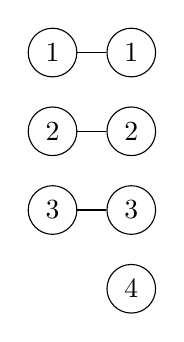
\begin{tikzpicture}[main/.style = {draw, circle},node distance=1cm and 0.5cm]
            \node[main] (1) {1};
            \node[main] (2)[below of=1] {2};
            \node[main] (3)[below of=2] {3};

            \node[main] (5)[right of=1] {1};
            \node[main] (6)[below of=5] {2};
            \node[main] (7)[below of=6] {3};
            \node[main] (8)[below of=7] {4};

            \draw (1) -- (5);
            \draw (2) -- (6);
            \draw (3) -- (7);

        \end{tikzpicture}
        \caption{$R_1$}
    \end{subfigure}
    \hfill
    \begin{subfigure}[b]{0.2\linewidth}
        \centering
        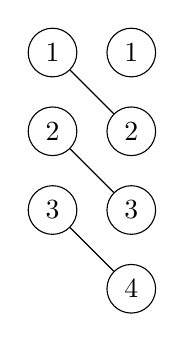
\begin{tikzpicture}[main/.style = {draw, circle},node distance=1cm and 2cm]
            \node[main] (1) {1};
            \node[main] (2)[below of=1] {2};
            \node[main] (3)[below of=2] {3};
            \node[main] (5)[right of=1] {1};
            \node[main] (6)[below of=5] {2};
            \node[main] (7)[below of=6] {3};
            \node[main] (8)[below of=7] {4};

            \draw (1) -- (6);
            \draw (2) -- (7);
            \draw (3) -- (8);

        \end{tikzpicture}
        \caption{$R_2$}
    \end{subfigure}
    \hfill
    \begin{subfigure}[b]{0.2\linewidth}
        \centering
        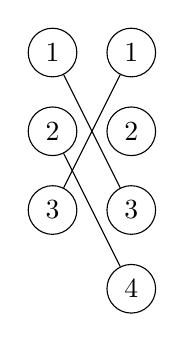
\begin{tikzpicture}[main/.style = {draw, circle},node distance=1cm and 2cm]
            \node[main] (1) {1};
            \node[main] (2)[below of=1] {2};
            \node[main] (3)[below of=2] {3};

            \node[main] (5)[right of=1] {1};
            \node[main] (6)[below of=5] {2};
            \node[main] (7)[below of=6] {3};
            \node[main] (8)[below of=7] {4};

            \draw (1) -- (7);
            \draw (2) -- (8);
            \draw (3) -- (5);

        \end{tikzpicture}
        \caption{$R_3$}
    \end{subfigure}
    \hfill
    \begin{subfigure}[b]{0.2\linewidth}
        \centering
        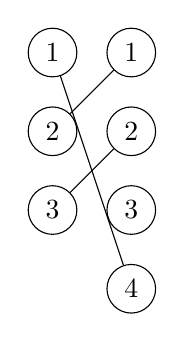
\begin{tikzpicture}[main/.style = {draw, circle},node distance=1cm and 2cm]
            \node[main] (1) {1};
            \node[main] (2)[below of=1] {2};
            \node[main] (3)[below of=2] {3};

            \node[main] (5)[right of=1] {1};
            \node[main] (6)[below of=5] {2};
            \node[main] (7)[below of=6] {3};
            \node[main] (8)[below of=7] {4};

            \draw (1) -- (8);
            \draw (2) -- (5);
            \draw (3) -- (6);

        \end{tikzpicture}
        \caption{$R_4$}
    \end{subfigure}


    \caption{Set \(\mathcal{R}\) for $M=3$ and $K=4$: $R_1$, $R_2$, $R_3$ and $R_4$ are, respectively, depicted in (a), (b), (c) and (d).}
    \label{fig:rr}
\end{figure}












\subsection{Warm-up: The $\HCLA$ Algorithm}

As previously pointed, the $\HCLA$ algorithm treats each $G \in \mathcal{G}$ as an individual super arm and maintains separate statistics including empirical mean $\hat{\mu}_{G}(t)$, KL-UCB index $d_G(t)$, and counters $N^\HCLA_G(t) = \abs{\mathcal{N}^\HCLA_G(t)}$ for each.
At each time step \(t\), the central decision maker selects a matching \(G(t)\) with the maximum empirical mean \(\hat \mu_G(t)\) and another matching \(\ghint_1(t)\) with the maximum KL-UCB $d_G(t)$ (Lines~\ref{line:empirical-G}--\ref{line:hint-G}).
Then, if the maximum KL-UCB $d_{\ghint(t)}(t)$ is greater than the maximum empirical mean \(\hat \mu_{G_t}(t)\), the central decision maker chooses \(\ghint(t)\) from the matching \(\ghint_1(t)\) or a uniformly random chosen matching \(\ghint_2(t)\) each with probability $\nicefrac{1}{2}$. It then asks for a hint from \(\ghint(t)\) and updates the empirical mean \(\hat \mu_{\ghint(t)}(t+1)\) according to the hint observation (Lines~\ref{l:line:klh}--\ref{line:end-query}).
Finally, the central decision maker selects the matching \(G(t)\) to pull and updates the empirical mean \(\hat \mu_{G(t)}(t+1)\) according to the reward observation of \(G(t)\) and updates KL-UCB $d_{G}(t+1)$ for all $G \in \mathcal{G}$ (Lines~\ref{line:pull-G}--\ref{line:update-mu-kl-ucb}).
The detailed pseudocode of the $\HCLA$ algorithm is provided in Algorithm \ref{routin:hcla}.

% and the agents pull the arms according to \(G(t)\).
% Every time there exists a matching $G' \neq G(t)$ such that $d_{G'}(t) > \hat{\mu}_{G(t)}(t)$, the central decision maker then sets one such matching $G'$ with the maximum $d_{G'}(t)$ to $\ghint(t)$, and agents ask for hints according to $\ghint(t)$ . The algorithm selects both $G(t)$ and $\ghint(t)$ by taking the maximum over the exponentially-sized set \(\mathcal{G}\).



\begin{algorithm}[tp]
    \caption{ Hinted Centralized Learning Algorithm ($\HCLA$) }\label{routin:hcla}

    \textbf{Input}: set of agents $\mathcal{M}=\{\text{central decision maker}\},\mathcal{K}=\mathcal{G},\mathcal{D},T$\\
    \textbf{Parameter}: $\hat{\mu}_{G}(t)\leftarrow 0, d_{G}(t)\leftarrow 0, \mathcal{N}_{G} = \emptyset$\\
    \begin{algorithmic}[1] 
        \For{$ t \in  [T]$}
        \State $G(t) \leftarrow \argmax_{G \in \mathcal{K}} \hat{\mu}_{G}(t)$ \label{line:empirical-G}
        \State $G'(t) \leftarrow \argmax_{G \in \mathcal{K}} d_{G}(t)$ \label{line:hint-G}
        \If{$d_{G'(t)}(t) > \hat{\mu}_{G(t)}(t)$} \label{l:line:klh}
        \State $G^{\textit{hint}}_1(t)\gets G'(t)$
        \State $\ghint_2(t) \gets$  pick a matching out of $\mathcal{G}$ uniformly at random \label{line:hint-choose-2}
        \State $\ghint(t) \gets
            \begin{cases}
                \ghint_1(t), & \text{w.p. } \frac{1}{2} \\
                \ghint_2(t), & \text{w.p. } \frac{1}{2}
            \end{cases}$ \label{line:1-2-hint-choose}

        \State Each agent $m$ asks for a hint from $k^{\ghint(t)}_m$
        \State Update $\hat{\mu}_{G^{\textit{hint}}(t)}(t+1)$ according to the observation of \(\ghint(t)\)
        \EndIf\label{line:end-query}
        \State Each agent $m$ pulls $k^G_m$ \label{line:pull-G}
        \State Update $\hat{\mu}_{G(t)}(t+1)$ according to the reward observation of \(G(t)\) 
        \State Update $d_{G}(t+1)$ for all $G\in\mathcal{G}$\label{line:update-mu-kl-ucb}
        \EndFor
    \end{algorithmic}
\end{algorithm}

Next, we present the upper bounds for the time-independent regret and the number of queried hints $L^\HCLA(T)$ for the $\HCLA$ algorithm in Theorem \ref{thm:matirphi}.
\begin{restatable}{theorem}{firsteuclid}\label{thm:matirphi}
    For $0< \delta < \frac{\Delta^G_{\min}}{2}$ and $\Delta_\delta = \mathrm{kl}(\mu_{G^*} - \Delta^G_{\min} + \delta, \mu_{G^*} - \delta)$, the $\HCLA$ algorithm has
    \begin{enumerate}
        \item time-independent $O\left(MK^{2M}\right)$ regret.
        \item  $L^\HCLA(T) \in O\left(\frac{MK^M \log T }{\Delta_\delta}\right).$
    \end{enumerate}
\end{restatable}


Although the regret of $\HCLA$ is time-independent, the exponential constants in the regret and hint upper bounds are rather unsatisfying. In what follows, we propose a new algorithm named $\GPHCLA$, which offers a more refined analysis while following the same hint inquiry and arm-pulling approach with a different usage of observations.


\subsection{The $\GPHCLA$ Algorithm}

We present $\GPHCLA$ in Algorithm~\ref{routin:hcla1}. This algorithm follows similar steps to $\HCLA$ in terms of identifying the empirically best matching $G(t)$ to pull and determining whether to ask for a hint. However, it employs a distinctly different approach for selecting $\ghint(t)$ and updating the statistics after each observation, whether pulling an arm or requesting a hint.
In this algorithm, the central decision maker maintains stats $\hat{\mu}_{m,k}(t)$ and $d_{m,k}(t)$ for each edge $(m,k) \in \mathcal{M} \times \mathcal{K}$, enabling it to run $\HALG$ algorithm \cite{kuhn1955hungarian} to find a matching $G(t)$ that maximizes the additive utility of any weighted bipartite graph (Line~\ref{line:hungarian-G}). This algorithm also identifies the hint graph $G'(t)$ by applying the same condition as $\HCLA$, but with a redefined $d_G(t) = \sum_{(m,k)\in G}d_{m,k}(t)$, allowing the decision maker to run $\HALG$ algorithm for hint inquiry as well (Line~\ref{line:hungarian-hint-G}).
Consequently, the algorithm determines $G(t)$ and $G'(t)$, with the output of $\HALG$ run over bipartite graph where the weight of the edges $(m,k)$ are $\hat{\mu}_{m,k}(t)$ and $d_{m,k}(t)$ respectively. Formally, $G(t)\gets\HALG(\bm{\hat{\mu}}(t))$  and $G'(t)\gets\HALG(\bm{d}(t))$, where $\bm{\mu},\bm{d} \in [0,1]^{M\times K}$ are the matrices of the corresponding statistics.

Next, we present the hint query mechanism of \(\GPHCLA\).
The algorithm first checks if the utility of the matching $G'(t)$ based on \(\bm d(t)\) is greater than that of the matching $G(t)$ based on \(\bm{ \hat{\mu}}(t)\), i.e., $U(G'(t),\bm{d}(t)) > U(G(t),\bm{\hat{\mu}}(t))$ (Line~\ref{line:hint-query}). 
If this condition holds, unlike $\HCLA$, which might query a hint the matching $G'(t)$ satisfying the hint inquiry condition, this algorithm \emph{projects} $G'(t)$ to a matching in the predefined set of pairwise edge-disjoint matchings $\mathcal{R}$. By projection, we mean mapping $G'(t) \in \mathcal{G}$ to a matching in $\mathcal{R}$, i.e., $\mathcal{G} \rightarrow \mathcal{R}$. For the projection step, the algorithm selects the matching $\ghint_1(t)$ from $\mathcal{R}$ that contains the edge $(m,k) \in G'(t)$ with the fewest number of observations $N^{\GPHCLA}_{m,k}(t)$ as well as another potential matching $\ghint_2(t)$ by selecting a matching from $\mathcal{R}$ uniformly at random (Lines~\ref{line:hint-choose-1}--\ref{line:hint-choose-2}).
The algorithm then sets $\ghint(t)$ to either $\ghint_1(t)$ or $\ghint_2(t)$ each with probability equal to $\nicefrac{1}{2}$. 
Each agent $m$ then ask for hints from their corresponding arms $k^{\ghint(t)}_m$.


\begin{algorithm}[tp]
    \caption{ Generalized Projection-based Hinted Centralized Learning Algorithm ($\GPHCLA$) }\label{routin:hcla1}
    \begin{algorithmic}[1]
        % \Input set of agents $\mathcal{M}$, set of arms  $\mathcal{K}$, time horizon $T$

        \State \textbf{initialization:} $\hat{\bm \mu}_{m}(t)\leftarrow \bm 0, \bm{d}_{m}(t)\leftarrow \bm 0, \bm{N}^{\GPHCLA}_{m} = \bm 0$ for each agent $m$

        \For{$t \in T$}


        \State $G(t) \leftarrow \HALG\left(\bm{\hat{\mu}}(t)\right)$
        \label{line:hungarian-G}

        \State $G'(t) \leftarrow \HALG\left(\bm{d}(t)\right)$\label{line:hungarian-hint-G}
        \If{$U(G'(t),\bm{d}(t)) > U(G(t),\bm{\hat{\mu}}(t))$}\label{line:hint-query}
        \State $( m,k ) \leftarrow \argmin_{(m',k') \in G'(t)}N^{\GPHCLA}_{m',k'}\left(t\right)$
        \State $\ghint_1(t) \leftarrow \{R\in \mathcal{R}: (m,k) \in R\}$ \label{line:hint-choose-1}
        \State $\ghint_2(t) \gets$  pick a matching out of $\mathcal{R}$ uniformly at random \label{line:hint-choose-2}
        \State $\ghint(t) \gets
            \begin{cases}
                \ghint_1(t), & \text{w.p. } \frac{1}{2} \\
                \ghint_2(t), & \text{w.p. } \frac{1}{2}
            \end{cases}$ \label{line:1-2-hint-choose}
        \State Each agent $m$ asks for a hint from $k^{\ghint(t)}_m$
        \label{line:end-hint-query}
        % \State Update
        \EndIf
        \State Each agent $m$ pulls $k^G_m$
        \State Update $\bm{\hat{\mu}}_m(t+1)$, \(\bm N^{\GPHCLA}_{m}\left(t+1\right)\), and $\bm {d}_m(t+1)$ for each agent $m$ according to new observations

        \EndFor
    \end{algorithmic}
\end{algorithm}


% As previously mentioned, $\GPHCLA$ keeps different stats at the edge level rather than at the matching level, as maintained by $\HCLA$. This approach enables the decision maker to run $\HALG$ algorithm, which has polynomial time complexity, rather than taking a maximum over an exponentially large set $\mathcal{G}$, which would result in a very slow algorithm. 

In Theorem \ref{thm:c_whhmmab}, we prove the bound of the regret and the asymptotically optimal bound for the number of hints.


\begin{restatable}{theorem}{secondeuclid}\label{thm:c_whhmmab}
    For $0< \delta < \frac{\Delta^G_{\min}}{2}$ and $\Delta_\delta=\mathrm{kl}(\mu_{G^*} - \Delta^\text{G}_{\min} + \delta, \mu_{G^*} - \delta)$, $\GPHCLA$ Algorithm~\ref{routin:hcla1} has
    \begin{enumerate}
        \item time-independent $O\left(M^4K\right)$ regret.
        \item hint complexity $L^{\GPHCLA}(T) \in O\left(\frac{MK \log T}{\Delta_\delta}\right)$.
    \end{enumerate}
\end{restatable}
Theorem \ref{thm:c_whhmmab} demonstrates the crucial effect of the edge-level decision-making approach utilized by $\GPHCLA$ on regret, reducing the exponential time-independent bound to a polynomial. Furthermore, it implies that the same hint inquiry approach augmented with projection, can significantly reduce the number of required hints such that the final bound for the number of hints is asymptotically optimal (matching the lower bound in Theorem~\ref{thm:hint-lower-bound}). 


\subsection{Analysis of \(\HCLA\) and $\GPHCLA$}
While \(\HCLA\) and \(\GPHCLA\) share the same arm-pulling and hinting procedures, their methods for selecting the hint graph \(\ghint\) and updating statistics differ. To avoid redundancy, we focus on \(\GPHCLA\) by providing the proof of Theorem \ref{thm:c_whhmmab}, which shows tighter bounds, and move the proof of Theorem \ref{thm:matirphi} to Appendix \ref{proof:hcla}. Additionally, we introduce an edge-level analysis for \(\GPHCLA\) that, unlike \(\HCLA\), considers how observations from a matching affect estimations of other matchings sharing an edge or subset of edges.

Our proofs use an \emph{event-based} analysis inspired by \cite{wang2020optimal}, which was originally developed for homogeneous multi-armed bandits. We adapt this approach to the heterogeneous setup, addressing the unique challenges it presents. Section \ref{eba} covers the general approach to event-based regret. Specifically, the event-based analysis relies on bounding the size of each set defined in Definition \ref{def:sets}.

\begin{restatable}{definition}{events}
\label{def:sets}
We define the following sets of time steps at which specific events occur as:
{
\footnotesize 

\begin{align*}
    \mathcal{A} & \coloneqq \{t \geq 1: G(t) \neq G^*\}\\ 
    \mathcal{B} & \coloneqq \{t \geq 1: \abs{U\left(G(t); \bm{\hat{\mu}}(t)\right) - U\left(G(t); \bm{\mu}\right)} \geq \delta\}\\ 
    \mathcal{C} & \coloneqq \{t \geq 1: U\left(G^*; \bm{d}(t)\right) < U\left(G^*; \bm{\mu}\right)\}\\
    \mathcal{D} & \coloneqq \{t \geq 1: t \in \mathcal{A} \setminus (\mathcal{B} \cup \mathcal{C}), \abs{U\left(G^*; \bm{\hat{\mu}}(t)\right) - U\left(G^*; \bm{\mu}\right)} \geq \delta\}\\
    \mathcal{E} &\coloneqq \{t \geq 1: U(G'(t), \bm{d}(t)) > U(G^*, \hat{\bm{\mu}}(t))\}
\end{align*}
}
\end{restatable}

Intuitively, \(\mathcal{A}\) contains the time steps at which a sub-optimal matching is pulled, incurring regret. We also need to bound the size of the set \(\mathcal{B}\), which includes the time steps where the chosen matching is not well-estimated, potentially leading to the selection of a sub-optimal \(G(t)\). The sets \(\mathcal{C}\) and \(\mathcal{D}\) help us bound the exploration needed to identify \(G^*\) through hints when a sub-optimal matching is selected. Finally, \(\mathcal{E}\) bounds the number of required hints when \(G^*\) is detected, to explore potential matchings that might not have been chosen as \(G(t)\) due to potentially inaccurate estimations.


% \subsubsection{Proof Sketch of Theorems \ref{thm:matirphi} and \ref{thm:c_whhmmab}} \label{proof:sketch}
% \hfill \break
According to Definition \ref{def:sets} We now can prove the Theorem~\ref{thm:c_whhmmab} with event-based analysis as follows:
\begin{proof}[Proof of Theorem \ref{thm:c_whhmmab}]

Using Lemma~\ref{lemma:proof1} we can write:
\begin{align*}
    R^\GPHCLA(T) &\leq M\left(\E\left[\abs{\mathcal{B}}\right]+\E\left[\abs{\mathcal{C}}\right]+\E\left[\abs{\mathcal{D}}\right]\right),\\
    &\overset{(a)}\leq 15M^2 + 4M^2K + 16M^2k^2 + 6M^4K\delta^{-2},
\end{align*}
where inequality (a) holds by aggregation over the results of Lemmas~\ref{lemma:proof2},~\ref{lemma:proof3}, and~\ref{lemma:proof4}.
Therefore, the total regret of \(\GPHCLA\) is included to be in \(O\left(M^4K\right)\). 

By directly applying the result of Lemma~\ref{lemma:proof5}, we can write
\begin{align*}
    L^\GPHCLA(T) &\leq M \sum_{G' \in \mathcal{G}} \E\left[\abs{\mathcal{E}_{G'}}\right],\\
    &\leq 4MK^3 + 2M^3K\delta^{-2} + \frac{2MK \log T}{\Delta_\delta},
\end{align*}
which implies that $L^\GPHCLA(T) \in O\left(\frac{MK \log T}{\Delta_\delta}\right)$ that wraps the proof up.
\end{proof}



We also analyze another variation of the $\HCLA$ algorithm, named $\GHCLA$, which represents a more natural extension of $\HCLA$ that does not project $G'(t)$ to a matching in $\mathcal{R}$. The $\GHCLA$ algorithm inquires for a matching $\ghint(t)$, which is either $G'(t)$ or $\ghint_2(t)$, each with probability $\nicefrac{1}{2}$. In Theorem \ref{lemma:hcla2} in the appendix, we prove that $\GHCLA$ queries for \(O\left(\frac{M^2K \log T}{\mathrm{kl}(\mu_{G^*} - \Delta^G_{\min} + \delta, \mu_{G^*} - \delta)}\right)\) hints, which can be $M$ times larger than that of $\GPHCLA$, highlighting the important role that projection plays.







\section{Algorithms for Decentralized Hinted Heterogeneous Multi-Armed Bandits} \label{routine:decgame}

We focus on designing learning algorithms for \emph{Decentralized Hinted Heterogeneous Multi-Armed Bandits} ($\D\_\HHMMAB$s). Unlike the centralized setup, there is no central decision maker to help agents learn $G^*$ and avoid collisions. However, agents are allowed to \emph{communicate} with each other, sharing their statistics such as $\bm{\hat{\mu}}$s. By Theorem \ref{obs:msg}, we demonstrate that it is impossible for any decentralized learning algorithm to achieve sub-linear regret without agents sharing their statistics in $\HHMMAB$s. Consequently, communication is a crucial element in designing algorithms for $D\_\HHMMAB$s. After all agents communicate and send their statistics to the others, they determine a matching \( G \in \mathcal{G} \) by running $\HALG$ on the gathered statistics, which they commit to until the next communication phase. The communication protocol involves agents intentionally colliding with the specific agent they wish to communicate with while all agents engage with their corresponding arms \( k^{G}_m \) in the matching \( G \in \mathcal{G} \) they have established since the last communication.





\begin{theorem}\label{obs:msg}
No decentralized learning algorithm can provide sub-linear instance-independent regret for $\HHMMAB$s without agents knowing the statistics of the others.
\end{theorem}

\begin{proof}
% [Proof of Theorem \ref{obs:msg}]
The proof demonstrates that not knowing the magnitudes of other agents' statistics causes more conflicts in the future because it is  impossible for agents to distinguish between different possible reward models using their private information.

Consider two instances, \(A\) and \(B\), with \(M=2\) and \(K=2\), where the sets of agents and arms are \(\mathcal{M} = \{m_1, m_2\}\) and \(\mathcal{K} = \{k_1, k_2\}\), respectively. We assume that the instances are:
\begin{align*}
A:&\bm{\mu}_{m_1} = \langle \frac{1}{2}+\epsilon,\frac{1}{2}-\epsilon\rangle \quad \bm{\mu}_{m_2} = \langle 2\epsilon,\epsilon\rangle\\
B:&\bm{\mu}_{m_1} = \langle \frac{1}{2}+\epsilon,\frac{1}{2}-\epsilon\rangle \quad \bm{\mu}_{m_2} = \langle 4\epsilon,\epsilon\rangle\\
\end{align*}
Any fixed policies $\pi_{m_1}$ and $\pi_{m_2}$ chosen by the agents that achieve sub-linear regret on instance \(A\) will fail on instance \(B\). 
The reason is that in instance \(A\), the optimal solution for agent \(m_1\) is to pull arm \(k_1\). 
This means that every time a conflict occurs on arm \(k_1\), policy $\pi_{m_1}$ chooses to keep requesting to pull arm $k_1$ while policy $\pi_{m_2}$ leads agent \(m_2\) to stop requesting $k_1$ and try to pull $k_2$ instead.

However, if the underlying instance is \(B\), agent \(m_1\)'s policy, $\pi_{m_1}$, still requests arm $k_1$ when a conflict on \(k_1\) occurs. 
The reason is that without knowing the magnitude of agent $m_2$'s utility, instances $A$ and $B$ are indistinguishable from $k_1$'s perspective. Therefore, agent \(m_1\) continues pulling arm \(k_1\) in instance \(B\) and $m_2$'s policy $\pi_{m_2}$ switches to request arm $k_2$ for the same reason. Meanwhile, the optimal matching under instance $B$ is for $m_1$ to pull $k_2$ and for $m_2$ to pull $k_1$, which leads policies $\pi_{m_1}$ and $\pi_{m_2}$ to a linear regret.
\end{proof}

To incorporate communication, we outline the framework for our proposed learning algorithms, \emph{Hinted Decentralized Explore-then-Commit} ($\HDETC$) and \emph{Elimination-Based Hinted Decentralized Explore-then-Commit} ($\EBHDETC$). These algorithms divide the time horizon into \emph{exploration} and \emph{communication} phases, querying for hints in an orderly round-robin manner from $\mathcal{R}$ if needed, replicating the explore-then-commit approach. The main difference between these algorithms lies in the stopping condition for hint inquiries: in $\HDETC$, agents are assumed to be aware of $\Delta^\text{G}_{\min}$, while $\EBHDETC$ uses elimination to relax this assumption, allowing the agents to proceed without knowing the minimum gap. We then explain how agents specify exploration and communication \emph{epochs} and explore during these phases using the potentially inaccurate statistics gathered from the previous communication phase.




\subsection{Decentralized Learning Framework}\label{routine:framework}
We present the common framework used by all algorithms for \(D_\HHMMAB\), discussed in the following sections. All algorithms generally divide the \(T\) decision-making rounds into exploration and communication phases, with each exploration epoch followed by a communication epoch and vice versa. Consequently, all learning algorithms maintain a counter \(\rho\) as an index for each exploration epoch, and with a slight abuse of notation, \(\mathcal{N}_{m,k}^\rho\) represents the set of time steps in which agent \(m\) has pulled or hinted at arm \(k\) up to the beginning of exploration epoch \(\rho\). Additionally, agents can query hints during both communication and exploration epochs. 


Another important variable is the epoch length \(b^\rho\). The length of each epoch can vary over time. For example, in \cite{shi2021heterogeneous}, the length of each epoch increases exponentially as time goes on, $O\left(\log T\right)$ number of epochs in total. However, in this work, we assume that \(b^\rho = K\) for all exploration epochs, leading to a total of \(\nicefrac{T}{K}\) exploration epochs.

The reason we do not adopt the exponentially extending epoch length approach used in some works, such as \cite{shi2021heterogeneous} and \cite{mehrabian2020practical}, is that event-based analysis, which is fundamental to our proofs, cannot achieve better than \(O(\log\log T)\) regret under such exploration models.


Our decentralized learning framework with communication for $\HHMMAB$ consists of several phases:
\begin{description}[leftmargin=0pt]

    \item[Initialization phase:] assigns unique ranks among the agents.
    \item[Exploration phase:] The agents use the gathered statistics to identify the empirically best matching $G^\rho$ up to the beginning of epoch $\rho$, using the $\HALG$ algorithm. They then commit to their corresponding arm $k^{G^\rho}_m$ for $2^{b^\rho}$ rounds until the end of the epoch. At the end of epoch $\rho$, agents signal the start of the communication phase by creating collisions on the arms being pulled by other agents.


    \item[Communication phase:] Agents first quantize their potentially decimal statistics $\bm{\hat{\mu}}$ and use collisions to transmit the information bits. A collision indicates a '1', while the absence of a collision indicates a '0'. This peer-to-peer communication occurs after sending a signal to initiate communication phase. Agents use their uniquely assigned ranks to identify the sender and receiver.


Hint inquiry is a key part of the algorithms we, however, agents can query a hint at every time step regardless of whether it is the exploration or communication phase.

\end{description}
\paragraph{Rank Assignment.}
\hfill \break
The rank assignment algorithm is adopted from \citet{wang2020optimal} and consists of two procedures: \emph{Orthogonalization} and \emph{Rank Assignment}. 
The orthogonalization procedure assigns each player a unique external rank \( k \in [K] \). It involves a series of blocks, each of length \( K+1 \). During the first time step of each block, players attempt to select arms without causing collisions. The results of these attempts (whether successful or not) are shared through communication.
In the rank assignment sub-phase, a modified Round-Robin hopping scheme helps players convert their external ranks to unique internal ranks \( m \in [M] \) and estimate the total number of players \( M \). In \cite{wang2020optimal} the authors proved that the expected duration of the rank assignment procedure is bounded by $\frac{K^2 M}{K-M} + 2 K$.  A detailed description and analysis of the rank assignment algorithm can be found in \cite{wang2020optimal}.



\paragraph{Communication Protocol.}
\label{routine:com}
\hfill \break
In decentralized multi-agent multi-armed bandit problems where direct communication is prohibited, agents can use collisions as signals to transmit bits, as proposed by \cite{boursier2019sic}. In this setup, players communicate sequentially: one player samples an arm while the other either pulls the same arm (creating a collision, represented by bit 1) or does not pull it (no collision, represented by bit 0) to convey a single bit of information. Although this method allows for information sharing, it is costly due to collisions, which can reduce the rewards obtained by the agents. The main challenge is to minimize information loss resulting from the \emph{integralization} of non-integer statistics and to keep the communication phase between agents as short as possible. Sharing arm statistics \(\hat{\mu}_{m,k}(t)\), which are typically precise decimals, is challenging given the digital communication protocol. Therefore, agents should transmit the quantized format of their statistics, \(\hat{\mu}_{m,k}(t)\), denoted as \(\tilde{\mu}_{m,k}(t)\), which other agents will use to make decisions over time. Additionally, we define \(\tilde{d}_{m,k}(t)\) as
$$
\tilde{d}_{m,k}(t) \coloneqq \sup \left\{ q \geq 0 : N_{m,k}(t)\ \mathrm{kl}\left(\tilde{\mu}_{m,k}(t), q\right) \leq f(t) \right\}.
$$
where $f(t) = \log t + 4 \log \log t.$

We also introduce \(\tilde{\mu}^\rho_{m,k}\) as the statistic of the edge \((m,k)\) that is shared among the agents while communicating before starting exploration epoch \(\rho\). To minimize information loss while optimizing the duration of communication for each statistic \(\bm{\hat{\mu}}\), we focus on the \textit{Differential} communication protocol introduced by \citet{shi2021heterogeneous}. In this protocol, agents transmit \(\tilde{\delta}^\rho_{m,k} \coloneqq \tilde{\mu}^\rho_{m,k} - \tilde{\mu}^{\rho-1}_{m,k}\) using \(\left\lceil 1 + \frac{\log \rho}{2} \right\rceil\) bits. Receivers then update their stored statistics with \(\tilde{\mu}^\rho_{m,k} = \tilde{\mu}^{\rho-1}_{m,k} + \tilde{\delta}^\rho_{m,k}\). \citet{shi2021heterogeneous} proved that 
\begin{align}
    \hat{\mu}_{m,k}^\rho &\leq \tilde{\mu}_{m,k}^\rho,\\
     \tilde{\mu}^{\rho}_{m,k} - \hat{\mu}^{\rho}_{m,k} &\leq \sqrt{\frac{1}{\rho}}, \label{ineq:comerr}
\end{align}
which are crucial for the analysis. They also demonstrated that transmitting \(\tilde{\delta}^\rho_{m,k}\) requires \(O(1)\) bits, providing an upper bound on the regret incurred by each peer-to-peer communication before each epoch. The duration of each communication phase is in $O\left(M^2K\right)$ because each statistic $\tilde{\mu}^\rho_{m,k}$ should be shared with $M$ agents.


\paragraph{Hint Inquiry Mechanism}
\hfill \break
Even though both $\HDETC$ and $\EBHDETC$ follow the same exploitation approach as $\HCLA$ \ref{routin:hcla}, they query for hints from matchings in $\mathcal{R}$ during each epoch in a round-robin manner, i.e., \( G^\text{hint}(t) = R_{t\%K} \). This approach implicitly incorporates an \emph{Explore-Then-Commit} (ETC) style of exploration. In contrast, $\HCLA$ queries for a hint only when needed. The main reason for using the ETC hinting approach is to avoid the continuous communication required by the hint inquiry method introduced in $\HCLA$. In $\HCLA$, hints are queried based on \(\bm{d}_G(t)\), which requires agents being aware of the statistics of others at each time step. This constant need for communication would result in linear regret, as agents would be communicating all the time. On the other hand, round-robin hinting for \( K \) consecutive rounds allows agents to gather information about the matchings without continuous communication. This method ensures that within \( K \) rounds, agents have covered all possible matchings \( G \in \mathcal{G} \), including a matching $\HCLA$ would query a hint for. Thus, round-robin hinting effectively balances exploration and communication, reducing the overall communication complexity while achieving time-independent regret.

\paragraph{Regret Decomposition}
\hfill \break
All phases described in the learning framework are executed in the $\HHMMAB$ setup through making collisions. These collisions result in agents pulling suboptimal arms, which consequently incurs regret. Therefore, we decompose the regret into
\begin{align}
    R^{\pi}(T) &= R^{\pi_{\text{rank}}}(T) + R^{\pi_{\text{exp}}}(T) + R^{\pi_{\text{com}}}(T)
\end{align}
to analyze each component separately. These terms respectively denote the regret caused by `rank assignment', `exploration', and `communication' under policy $\pi$.

\subsection{Warm-Up: The $\HDETC$ algorithm}
As noted above, the $\HDAC$ algorithm follows the learning framework described in Section \ref{routine:framework} up to the time step \( t' \), which will be set later, with each exploration epoch having a fixed length equal to \( K \), i.e., \(\forall \rho > 0, 2^{b^\rho} = K\). Under the hint inquiry mechanism of the $\HDETC$ algorithm, each agent queries a hint from their corresponding arm in \( R_{t\%K} \in \mathcal{R} \), i.e., \( k^{R_{t\%K}}_m \), up to time step \( t' \). Agents then signal to start the new and final communication phase to gather \(\tilde{\mu}_{m,k}(t')\). Next, agents run $\HALG\left(\bm{\tilde{\mu}}(t')\right)$ to determine the matching \( G'^* \) to commit to for the remainder of the time, i.e., \(\forall t > t', G(t) = G'^* \). By Theorem \ref{thm:hdetc}, we proved that setting a proper $t'$ requires the agents to know $\Delta^\text{G}_{\min}$. 




\begin{algorithm}[t]
\caption{ Hinted Decentralized Explore then Commit ($\HDETC$) : agent $m$}\label{routin:hdetc}
\begin{algorithmic}[1]
\Input agent rank \(m\), arm set \(\mathcal{K}\), total number of agent \(M\), time threshold for hint inquiry $t'$ 
\State \textbf{Initialization:} epoch index $\rho \leftarrow 0$, 
 time index $t \leftarrow 0$, mean estimates $\hat{\mu}_{m,k}(t)\leftarrow 0, \tilde{\mu}_{m,k}^\rho \leftarrow 0$ for all $(m, k)$, set of times slots $ \mathcal{N}_{m,k}(t) \gets \emptyset$
 
 % , communication bit number $ b_{m, k}^\rho \leftarrow \left\lfloor\log _2\left(N_{m,k}(t)\right)\right\rfloor$, for all arms $k$
\If{$t < t'$}
\For{each epoch \(\rho\) }
%\State $ b_{m, k}^\rho \leftarrow \left\lfloor\log _2\left(N_{m,k}(t)\right)\right\rfloor$, for all arms $k$

\State $G^\rho \gets \HALG\left(\bm{\tilde{\mu}}^\rho\right)$ 
\State $ t_0 \gets t$
\LeftComment{Arm pulling}
\For{\(t \le t_0 + K\)}\label{line:hd-etc-reuse-begin}
\State Pull the arm $k^{G^{\rho}}_m$
\State Update $\hat{\mu}_{m,k^{G\rho}_m(m)}(t+1)$
\LeftComment{Hint query}
\State Ask for a hint from $k^{R_{t\%K}}_m$
\State Update $\hat{\mu}_{m,k^{R_{t\%K}}_m}(t+1)$


\State $t \leftarrow t + 1$
\EndFor 
\LeftComment{Communicate and update mean estimates}
\For{ $k \in [K]$ } 

\State $\tilde{\delta}_{m, k}^{\rho+1} \gets \tilde{\mu}^{\rho+1}_{m,k} - \tilde{\mu}^{\rho}_{m,k}$
\State $\operatorname{Send2All(\tilde{\delta}_{m, k}^{\rho+1})}$

\EndFor
\State $\rho \gets \rho + 1$ 
\State $t \gets t + \text{Communication 
 Time}$ \label{line:hd-etc-reuse-end}
\EndFor
\EndIf
\State $G'^* \gets  \HALG\left(\bm{\tilde{\mu}}^\rho\right)$
\While{$t \leq T$}
\State Pull the arm $k^{G'^*}_m$
\EndWhile
\end{algorithmic}
\end{algorithm}


\begin{theorem} \label{thm:hdetc}
For $t' = \frac{9M^2K \log(2MT)}{(\Delta^{G}_{\min})^2}$, the $\HDETC$ algorithm has
\begin{enumerate}
    \item time-independent $R^{\HDETC_{\text{exp}}}(T) \in O\left(M^3K^2\right)$.
    \item $R^{\HDETC_{\text{com}}}(T) \in \Theta\left(M^2t'\right)$.
    \item $L^{\HDETC}(T) \in \Theta\left(Mt'\right)$
\end{enumerate}

\end{theorem}

Although $\HDETC$ achieves time-independent exploration regret with logarithmic upper bounds for both communication regret and the number of queried hints, it assumes that agents are aware of $\Delta^\text{G}_{\min}$, which is generally considered an unrealistic assumption. Therefore, we propose a new elimination-based algorithm, $\EBHDETC$ (Algorithm \ref{routin:ebhdetc}), which attains the same bound without requiring agents to know the minimum gap.



\subsection{The $\EBHDETC$ algorithm }

In $\EBHDETC$, agents use a different approach to stop hinting which relaxes the assumption of having the minimum gap $\Delta^\text{G}_{\min}$ as a known parameter. Specifically, each agent maintains a set of active edges named $\mathcal{C}^\rho$, which contains all the edges that still have the odds to be included by in $G^\rho$ in the forthcoming epoch $\rho$. This set contains all the edges at the beginning, i.e. $C^1 = \{ (m,k) \in \mathcal{M}\times \mathcal{K}\}$. We avoid using agentwise subscripts for $\mathcal{C}^\rho$ because it is the same among all the agents. Agents decide the edges to be eliminated from $\mathcal{C}^\rho$ based on an error variable $\epsilon^\rho$ defined as $\epsilon^\rho \coloneqq \sqrt{\frac{\log\left(\frac{2}{\eta}\right)}{\rho}},$
with $\eta = \sqrt{\frac{2}{MT^2}}$.

In the $\EBHDETC$ algorithm, agents use this error variables to define a decisive condition to stop hinting, rather than using $t < t'$ as in $\HDETC$. Specifically, agents follow the same learning framework as $\HDETC$ but use a completely different criterion for entering the exploitation phase. Additionally, under $\EBHDETC$, agents determine $G^\rho$ at the beginning of each epoch $\rho$. The agents then utilize $\mathcal{C}^\rho$ to check for the existence of a matching $G^\rho_{(m,k)} \neq G^\rho$ such that
$$U(G^\rho, \bm{\tilde{\mu}}^\rho) - U(G^\rho_{(m,k)}, \bm{\tilde{\mu}}^\rho) \leq 4M \bm{\epsilon}^\rho,$$
where each $G_{(m,k)}^\rho$ is constructed as 
\[G_{(m,k)}^\rho \coloneqq \{(m,k)\} \cup \HALG\left(\bm{\tilde{\mu}}^\rho_{-m,-k}\right),\]
for all $(m,k) \in \mathcal{C}^\rho$, with $\bm{\tilde{\mu}}^\rho_{-m,-k}$ denoting the matrix $\bm{\tilde{\mu}}^\rho$ after the removal of row $m$ and column $k$. If there is no such $G_{(m,k)}^\rho$, agents stop communicating and hinting and commit to $G^\rho$ for the remainder of the time. Otherwise, agents eliminate the edges $(m,k) \in \mathcal{C}^\rho$ whose corresponding $G^\rho_{(m,k)}$ does not satisfy 
\[U(G^\rho; \bm{\tilde{\mu}}^\rho) - U(G^\rho_{(m,k)}; \bm{\tilde{\mu}}^\rho) \leq 4M \bm{\epsilon}^\rho\]
to update $\mathcal{C}^{\rho+1}$ and continue pulling $k_m^{G^\rho}$ and querying hints for $k_m^{R_{t\%K}}$ until the end of the epoch.


\begin{algorithm}[H]
\caption{ Elimination-Based Hinted Decentralized Explore then Commit ($\EBHDETC$) : agent $m$}\label{routin:ebhdetc}
\begin{algorithmic}[1]
\Input agent rank \(m\), arm set \(\mathcal{K}\), total number of agent \(M\), time threshold for hint inquiry $t'$ 
\State \textbf{Initialization:} epoch index $\rho \leftarrow 0$, 
 time index $t \leftarrow 0$, mean estimates $\hat{\mu}_{m,k}(t)\leftarrow 0, \tilde{\mu}_{m,k}^\rho \leftarrow 0$ for all $(m, k)$, set of times slots $ \mathcal{N}_{m,k}(t) \gets \emptyset$, set of active edges $\mathcal{C}^\rho \gets \{(m,k) \in \mathcal{M} \times \mathcal{K}\}$
 
 % , communication bit number $ b_{m, k}^\rho \leftarrow \left\lfloor\log _2\left(N_{m,k}(t)\right)\right\rfloor$, for all arms $k$

\While{$\abs{\mathcal{C}^{\rho}} > M$}
%\State $ b_{m, k}^\rho \leftarrow \left\lfloor\log _2\left(N_{m,k}(t)\right)\right\rfloor$, for all arms $k$





\LeftComment{Decide the committed matching in the epoch}
\State $G^\rho \gets \HALG\left(\bm{\tilde{\mu}}^\rho\right)$ 

\State $ \mathcal{C}^{\rho+1} \gets \emptyset$
\For{ $(m,k) \in \mathcal{C}^\rho$}
\State $G_{(m,k)}^\rho \gets (m,k) \cup \HALG\left(\bm{\tilde{\mu}}^\rho_{-m,-k}\right)$
\If{$U(G^\rho; \bm{\tilde{\mu}}^\rho) - U(G^\rho_{(m,k)}; \bm{\tilde{\mu}}^\rho) \leq 4M \bm{\epsilon}^\rho$}
\State $ \mathcal{C}^{\rho+1} \gets \mathcal{C}^{\rho+1} \cup (m,k)$
\EndIf
\EndFor

\State Execute Lines~\ref{line:hd-etc-reuse-begin}-\ref{line:hd-etc-reuse-end} of Algorithm~\ref{routin:hdetc}
% \LeftComment{Arm pulling}
% \For{$K$ rounds}
% \State Pull the arm $k^{G^{\rho}}_m$
% \State Update $\hat{\mu}_{m,k^{G\rho}_m(m)}(t+1)$
% \LeftComment{Hint query}
% \State Ask for a hint from $k^{R_{t\%K}}_m$
% \State Update $\hat{\mu}_{m,k^{R_{t\%K}}_m}(t+1)$


% \State $t \leftarrow t + 1$
% \EndFor 
% \LeftComment{Communicate and update mean estimates}
% \For{ $k \in [K]$ } 

% \State $\tilde{\delta}_{m, k}^\rho \leftarrow \tilde{\mu}^{\rho}_{m,k} - \tilde{\mu}^{\rho-1}_{m,k}$
% \State $\operatorname{Send2All(\tilde{\delta}_{m, k}^\rho)}$

% \EndFor
% \State $\rho \gets \rho + 1$
% \State $t \gets t + \text{Communication 
%  Time}$

\EndWhile
\LeftComment{Exploitation Phase}
\State Pull the arm $k^{G_{\mathcal{C}^\rho}}_m$ for the rest of the time
\end{algorithmic}
\end{algorithm}

\begin{theorem} \label{thm:ebhdetc}
For $\rho' \leq \frac{64M^2\log\left(T\sqrt{2M}\right)}{\left(\Delta^\text{G}_{\min}\right)^2}$, the $\EBHDETC$ algorithm has
\begin{enumerate}
    \item time-independent $R^{\EBHDETC_{\text{exp}}}(T) \in O\left(M^3K^2\right)$.
    \item communication regret $R^{\EBHDETC_{\text{com}}}(T) \in O\left(M^2K\rho'\right)$.
    \item hint complexity $L^{\EBHDETC}(T) \in O\left(MK\rho'\right)$
\end{enumerate}
\end{theorem}


\subsection{Analysis of \(\HDETC\) and $\EBHDETC$}\label{proof:sketch}


 

According to \cite{wang2020optimal}, the regret caused by the rank assignment phase, which follows the same routine in both algorithms, has a time-independent upper bound. They showed that
\[
R^{\pi_{\text{rank}}}(T) \leq M\left(\frac{K^2 M}{K-M} + 2 K\right).
\]

Furthermore, \citet{shi2021heterogeneous} demonstrated that the \textit{Differential} protocol requires \(O(1)\) bits for each peer-to-peer communication to transmit at each epoch. This protocol induces \(O(M^2K)\) regret at each communication phase, where \(M^2K\) is the total number of statistics shared among agents at each communication phase. However, unlike the rank assignment phase, which is common among all algorithms, different policies may have different exploration epoch lengths, leading to varying numbers of communication phases. Therefore, we aim to analyze \(R^{\pi_{\text{exp}}}(T) + R^{\pi_{\text{com}}}(T)\) while maintaining a time-independent upper bound for \(R^{\pi_{\text{exp}}}(T)\) with the minimum possible hints.

 
\begin{proof}[Proof of Theorem \ref{thm:hdetc}]
    
   First, we argue that \(L^{\HDETC}(T) \in O\left(\frac{M^3K \log(2MT)}{(\Delta^\text{G}_{\min})^2}\right)\) because agents request \(M\) hints during the first \(t'\) rounds.
   
   We then bound \(R^{\HDETC_{\text{com}}}(T)\). In $\HDETC$, agents communicate every \(k\) rounds up to time step \(t'\) and only once after that. Therefore, we can conclude that \(R^{\HDETC_{\text{com}}}(T) \in O\left(M^2t'\right)\).

The \(\HDETC\) algorithm has \(\frac{t'}{K}\) decision-making rounds up to the time step \(t'\), followed by one additional round for the period from \(t'\) to \(T\). Thus, we can break down the exploration regret of \(\HDETC\) as follows:
\[ R^{\HDETC_{\text{exp}}}(T) = R^{\HDETC_{\text{exp}}}(t') + R^{\HDETC_{\text{exp}}}(t':T) .\]


We then apply the results of Lemma \ref{lemma:deba} to bound \(R^{\HDETC_{\text{exp}}}(t')\) as:
\begin{align*}
R^{\HDETC_{\text{exp}}}(t') \leq 19M^2K + 4M^2K^2 \\+ \left(4M^3K + 8M^4K + 8M^4K^2\right)\delta^{-2}. 
\end{align*}

To further bound \( R^{\HDETC_{\text{exp}}}(t':T) \), we write:
\begin{align*}
R^{\HDETC_{\text{exp}}}(t':T) & \leq 0T \Pr\left(G'^* = G^*\right) + MT \Pr\left(G'^* \neq G^*\right), \\
& \leq MT \Pr\left(G'^* \neq G^*\right), \\
& \overset{(a)}{\leq} M,
\end{align*}
where the inequality holds by Lemma \ref{lemma:main-hdetc}, which bounds the probability of \(G'^* \neq G^*\).

Therefore, we can write:
\begin{align}
R^{\HDETC_{\text{exp}}}(T) \leq M+19M^2K + 4M^2K^2 \nonumber\\+ \left(4M^3K + 8M^4K + 8M^4K^2\right)\delta^{-2}.
\end{align}
which results in a time-independent exploration regret.

\end{proof}

\begin{proof}[Proof of Theorem \ref{thm:ebhdetc}]
Assuming \(\rho'\) as the index of the last exploration epoch during which agents, under both policies, query for hints for \(K\) consecutive rounds and then immediately start the communication phase, we can argue that \(L^\pi(T) = MK\rho'\) and \(R^{\pi_{\text{com}}}(T) \in O\left(M^2K\rho'\right)\).

While the hinting approach remains the same as in \(\HDETC\), in \(\EBHDETC\), we assume that the agents are unaware of \(\Delta^\text{G}_{\min}\), thus preventing them from querying for hints as in \(\HDETC\). Instead, under \(\EBHDETC\), agents maintain a set of active edges \(\mathcal{C}^\rho\), which includes the edges that could potentially be part of \(G^*\). Agents decide to stop hinting at the beginning of epoch \(\rho\) when \(\abs{\mathcal{C}^\rho} = M\). Consequently, \(\rho'\) becomes a random variable, as opposed to the fixed \(t'\) in \(\HDETC\). Regarding exploration regret, we can directly apply the bound established in Lemma \ref{lemma:deba}. Therefore, we focus on bounding \(R^{\EBHDETC_{\text{com}}}(T)\) and \(L^\EBHDETC(T)\), noting that the latter is \(MK\) times larger than the former due to the nature of the algorithm.

We, then, break down the exploration regret of \(\HDETC\) as follows:
{\footnotesize
\[ R^{\EBHDETC_{\text{exp}}}(T) = R^{\EBHDETC_{\text{exp}}}(K\rho') + R^{\EBHDETC_{\text{exp}}}(K\rho':T) ,\]
}
where $R^{\EBHDETC_{\text{exp}}}(K\rho')$ follows the same bound we proved in Lemma \ref{lemma:deba}. 

So we focus on bounding $R^{\EBHDETC_{\text{exp}}}(K\rho':T)$. Accordingly, we define the event $\mathcal{H}_T$ as
{\footnotesize 
\[
\mathcal{H}_{T}\coloneqq \mathds{1}\left\{\forall \rho \leq \frac{T}{K}, \forall G \in \mathcal{G}:\abs{U(G;\bm{\tilde{\mu}}^\rho) - U(G;\bm{\mu})} \leq 2M\epsilon^\rho\right\}.
\]
}
In Lemma \ref{lemma:ht}, we prove that \(\Pr\left(\mathcal{H}_T \neq 1\right) \leq \frac{1}{T}\).
Next, we focus on bounding the probability of $G_{\mathcal{C}^{\rho'}} = G^*$ to find an upper bound for $R^{\EBHDETC_{\text{exp}}}(K\rho':T)$. In Lemma \ref{lemma:matching}, we prove that the edges in the set of active edges when $\abs{\mathcal{C}^{\rho'}} = M$ forms a perfect matching and given $\mathcal{H}_T = 1$, the graph formed by the edges in $\mathcal{C}^{\rho'}$ is exactly $G^*$. Thus, we can imply that $\Pr\left(G_{\mathcal{C}^{\rho'}} \neq G^*\right) \leq \frac{M}{T}$.

By Lemma \ref{lemma:finale}, we can prove that given $\mathcal{H}_T = 1$, the index of final epoch $\rho' \leq \frac{64M^2\log\left(T\sqrt{2M}\right)}{\left(\Delta^\text{G}_{\min}\right)^2}$ and $G_{\mathcal{C}^{\rho'}} = G^*$. Thus, we write
\(
    R^{\EBHDETC_{\text{exp}}}(K\rho':T) \leq MT\Pr\left(\mathcal{H}_T = 0\right) + 0T\Pr\left(\mathcal{H}_T = 1\right) \leq M.
\)
Finally, 
\begin{align*}
    R^{\HDETC_{\text{exp}}}(T) \leq M+19M^2K + 4M^2K^2\\ + \left(4M^3K + 8M^4K + 8M^4K^2\right)\delta^{-2}.
\end{align*}
We wrap the proof up by applying the result of Lemma \ref{lemma:finale} to bound \(L^\pi(T) \in O\left(\frac{M^3K\log\left(T\sqrt{2M}\right)}{\left(\Delta^\text{G}_{\min}\right)^2}\right)\) and  \(R^{\pi_{\text{com}}}(T) \in O\left(\frac{M^4K\log\left(T\sqrt{2M}\right)}{\left(\Delta^\text{G}_{\min}\right)^2}\right)\).
\end{proof}



\section{Optimality of the Results}
\subsection{A Lower Bound on the Necessary Number of Hints}
Another important concern in designing efficient learning policies for $\HHMMAB$, is the number of queried hints $L^\pi(T)$. In Theorem \ref{thm:imphi}, we prove that all uniformly fast convergent learning policies, defined in Definition \ref{def:ufc}, require $\Omega(\log T)$ hints to achieve time-independent regret.  Accordingly, we call a policy $\pi$,  \textit{asymptotically hint optimal} if $L^\pi(T) \in O(\log T)$.
\begin{definition}\label{def:ufc}
    A policy $\pi$ is called uniformly fast convergent if for all $0<\alpha<1$ and all sub-optimal matchings $G \neq G^*$, $$\E\left[N^{\pi}_{G}(T)\right]=o\left(T^\alpha\right),$$ 
    holds.
\end{definition}
\begin{theorem}\label{thm:imphi}\label{thm:hint-lower-bound}
    Any uniformly fast convergent policy $\pi$ with time-independent regret should query for $L^\pi(T) \in \Omega(\log T)$ hints.
\end{theorem}
\begin{proof}
% [Proof of Theorem \ref{thm:imphi}]
Recall that in classic multi-armed bandits \cite{garivier2019explore,lai1985asymptotically}, for any uniformly fast convergent policy $\pi$, we have

$$
\liminf _{T \rightarrow \infty} \frac{\E\left[N_{G}^{\pi}\left(T\right)\right]}{\log T} \geqslant \frac{1}{\mathrm{kl}\left(U(G;\bm{\mu}), U(G^*;\bm{\mu})\right)}, \forall G \neq G^*,
$$

If the number of hints is $o(\log T)$, then there must be at least $\Omega(\log T)$ non-hint observations on some suboptimal arms. Consequently, for any uniformly fast convergent policy, the regret is also $\Omega(\log T)$, which is time-dependent.

\end{proof}



\subsection{A Lower Bound on the Necessary Number of Communications}

\section{Experiments}

\bibliography{abb,aaai25}
\appendix
\appendix

\section*{APPENDIX}
\onecolumn
\section{Communication Protocols}

\section{Algorithm $\GHCLA$}
Here we analyse hint complexity of algorithm $\GHCLA$ that is a variation of $\HCLA$. In this algorithm the super arm satisfying $U(G'(t);d(t)) > U(G(t);\hat{\mu}(t))$ would be served as $\ghint(t)$ with probability $\nicefrac{1}{2}$. In this section, we prove that $\GHCLA$ asks for at most \(O\left(\frac{M^2K \log T}{\mathrm{kl}(\mu_{G^*} - \Delta^\text{G}_{\min} + \delta, \mu_{G^*} - \delta)}\right)\) hints.
\begin{algorithm}[H]
\caption{ Generalized Centralized Learning Algorithm ($\GHCLA$)}\label{routin:hcla2}
\begin{algorithmic}[1]
% \Input set of agents $\mathcal{M}$, set of arms  $\mathcal{K}$, time horizon $T$

        \State \textbf{initialization:} $\hat{\bm \mu}_{m}(t)\leftarrow \bm 0, \bm{d}_{m}(t)\leftarrow \bm 0, \bm{N}^{\GHCLA}_{m} = \bm 0$ for each agent $m$

        \For{$t \in T$}


        \State $G(t) \leftarrow \HALG\left(\bm{\hat{\mu}}(t)\right)$
        

        \State $G'(t) \leftarrow \HALG\left(\bm{d}(t)\right)$
        \If{$U(G'(t),\bm{d}(t)) > U(G(t),\bm{\hat{\mu}}(t))$}
       
        \State $\ghint_1(t) \gets G'(t)$ 
        \State $\ghint_2(t) \gets$  pick a matching out of $\mathcal{R}$ uniformly at random \label{line:hint-choose-2}
        \State $\ghint(t) \gets
            \begin{cases}
                \ghint_1(t), & \text{w.p. } \frac{1}{2} \\
                \ghint_2(t), & \text{w.p. } \frac{1}{2}
            \end{cases}$ 
        \State Each agent $m$ asks for a hint from $k^{\ghint(t)}_m$
        
        % \State Update
        \EndIf
        \State Each agent $m$ pulls $k^G_m$
        \State Update $\bm{\hat{\mu}}_m(t+1)$, \(\bm N^{\GHCLA}_{m}\left(t+1\right)\), and $\bm {d}_m(t+1)$ for each agent $m$ according to new observations

        \EndFor
\end{algorithmic}
\end{algorithm}

\begin{restatable}{theorem}{secondeuclid1}\label{lemma:hcla2}
    For $0< \delta < \frac{\Delta^G_{\min}}{2}$ and $\Delta_\delta=\mathrm{kl}(\mu_{G^*} - \Delta^\text{G}_{\min} + \delta, \mu_{G^*} - \delta)$, $\GHCLA$ Algorithm~\ref{routin:hcla2} has
    \begin{enumerate}
        \item time-independent $O\left(M^4K\right)$ regret.
        \item hint complexity $L^{\GHCLA}(T) \in O\left(\frac{M^2K \log T}{\Delta_\delta}\right)$.
    \end{enumerate}
\end{restatable}

\begin{proof}[Proof of Theorem \ref{lemma:hcla2}]
The main difference between \(\GPHCLA\) and \(\GHCLA\) is the hint inquiry approach while the same event is triggered. Thus, the regret analysis for both algorithms is the same, while the number of hints is \(M\) times larger for \(\GHCLA\).

Now, to bound the hint complexity, we use the same set of moments \(\mathcal{E}_{G'}\) previously defined in the proof of Theorem \ref{thm:c_whhmmab} and define new sets of moments \( \mathcal{E}_{1,G'}\ \text{and } \mathcal{E}_{2,G'}\) as:


\begin{align*}
\mathcal{E}_{1,G'} &\coloneqq \{t \in \mathcal{E}_{G'}: \abs{U\left(G';\bm{\hat{\mu}}(t)\right) - U\left(G';\bm{\mu}(t)\right)} \geq \delta\},\\
\mathcal{E}_{2,G'} &\coloneqq \{t \in \mathcal{E}_{G'}: \sum_{t' = 1}^{t} \mathds{1}_{\{t' \in \mathcal{E}_{G'}\}} < t_0 \},\\
\mathcal{E}'_{1,G'} &\coloneqq \left\{t \in \mathcal{E}_{G'}: \exists  (m,k) \in G', \abs{\hat{\mu}_{m,k}(t) - \mu_{m,k}} \geq \frac{\delta}{M}\right\},\\
\mathcal{X}_{1,m,k} &\coloneqq \left\{t \geq 1: ( m,k ) \in G'(t), \abs{\hat{\mu}_{m,k}(t) - \mu_{m,k}} \geq \frac{\delta}{M}\right\},\\
\mathcal{X}_{2,m,k} &\coloneqq \left\{t \geq 1: \sum_{t' = 1}^{t} \mathds{1}\left\{(m,k) \in G'(t)\right\} < t_0\right\}.
\end{align*}
As argued in the proof of Theorem \ref{thm:c_whhmmab}, we know that \(\mathcal{E}_{G'} \subseteq \mathcal{E}_{1,G'} \cup \mathcal{E}_{2,G'} \).Then, we can conclude that 
$\E\left[\abs{\mathcal{E}_{1,G'}}\right] \leq \E\left[\abs{\mathcal{E}'_{1,G'}}\right],$ and also \[
\sum_{G' \in \mathcal{G}}\E\left[\abs{\mathcal{E}_{2,G'}}\right] \leq \sum_{(m,k) \in \mathcal{M} \times \mathcal{K}} \E\left[\abs{\mathcal{X}_{2,m,k}}\right].
\]

Therefore, we finish the proof by writing:

\begin{align*}
    \sum_{G' \in \mathcal{G}} \E\left[\abs{\mathcal{E}_{G'}}\right] 
    &\leq \sum_{G' \in \mathcal{G}} \E\left[\abs{\mathcal{E}_{1,G'}}\right] + \E\left[\abs{\mathcal{E}_{2,G'}}\right] \\
    &\leq \sum_{G' \in \mathcal{G}} \E\left[\abs{\mathcal{E}'_{1,G'}}\right] + \E\left[\abs{\mathcal{E}_{2,G'}}\right] \\
    &\overset{(a)}{\leq} \E\left[\sum_{G' \in \mathcal{G}} \abs{\mathcal{E}'_{1,G'}}\right] + \sum_{G' \in \mathcal{G}} \E\left[\abs{\mathcal{E}'_{2,S}}\right] \\
    &\overset{(b)}{\leq} \E\left[\sum_{t = 0}^T \sum_{G' \in \mathcal{G}} \mathds{1}\left\{G'(t) = G', \exists (m,k) \in G': \abs{\hat{\mu}_{m,k}(t) - \mu_{m,k}} \geq \frac{\delta}{M}\right\}\right] + \sum_{G' \in \mathcal{G}} \E\left[\abs{\mathcal{E}_{2,G'}}\right] \\
    &\overset{(c)}{\leq} \E\left[\sum_{(m,k) \in \mathcal{M} \times \mathcal{K}} \abs{\mathcal{X}_{1,m,k}}\right] + \sum_{G' \in \mathcal{G}} \E\left[\abs{\mathcal{E}_{2,G'}}\right] \\
    &\overset{(d)}{\leq} \sum_{(m,k) \in \mathcal{M} \times \mathcal{K}} \E\left[\abs{\mathcal{X}_{1,m,k}}\right] + \sum_{G' \in \mathcal{G}} \E\left[\abs{\mathcal{E}_{2,G'}}\right] \\
    &\leq \sum_{( m,k) \in \mathcal{M} \times \mathcal{K}} \E\left[\abs{\mathcal{X}_{1,m,k}}\right] + \E\left[\abs{\mathcal{X}_{2,m,k}}\right] \\
    &\leq 4MK + \frac{2M^3 K}{\delta^2} + \frac{2MK \log T}{\Delta_\delta}.
\end{align*}

while inequalities (a) and (d) hold because of the linearity of expectation. Inequality (b) is derived from the nature of the algorithm, which only chooses one \(G' \in \mathcal{G}\) to be hinted at each round. Another important observation is that when a super arm \(H_t\) is hinted at, there might be more than one edge \((m,k)\) satisfying \(\abs{\hat{\mu}_{m,k}(t) - \mu_{m,k}} \geq \frac{\delta}{M}\), which directly implies (c).


\end{proof}






\section{Event-Based Regret Analysis} \label{eba}

defining the following set of events
\begin{align*}
    \mathcal{A} & \coloneqq \{t \geq 1: G(t) \neq G^*\}\\ 
    \mathcal{B} & \coloneqq \{t \geq 1: \abs{U\left(G(t); \bm{\hat{\mu}}(t)\right) - U\left(G(t); \bm{\mu}\right)} \geq \delta\}\\ 
    \mathcal{C} & \coloneqq \{t \geq 1: U\left(G^*; \bm{d}(t)\right) < U\left(G^*; \bm{\mu}\right)\}\\
    \mathcal{D} & \coloneqq \{t \geq 1: t \in \mathcal{A} \setminus (\mathcal{B} \cup \mathcal{C}), \abs{U\left(G^*; \bm{\hat{\mu}}(t)\right) - U\left(G^*; \bm{\mu}\right)} \geq \delta\}\\
    \mathcal{E} &\coloneqq \{t \geq 1: U(G'(t), \bm{d}(t)) > U(G^*, \hat{\bm{\mu}}(t))\}
\end{align*}


Intuitively, \(\mathcal{A}\) contains the time steps at which a sub-optimal matching is pulled, incurring regret. We also need to bound the size of the set \(\mathcal{B}\), which includes the time steps where the chosen matching is not well-estimated, potentially leading to the selection of a sub-optimal \(G(t)\). The sets \(\mathcal{C}\) and \(\mathcal{D}\) help us bound the exploration needed to identify \(G^*\) through hints when a sub-optimal matching is selected. Finally, \(\mathcal{E}\) bounds the number of required hints when \(G^*\) is detected, to explore potential matchings that might not have been chosen as \(G(t)\) due to potentially inaccurate estimations.

We can then observe that for policy $\pi \in \{\HCLA,\GHCLA,\GPHCLA\}$,
\[ R^\pi(T) \leq M\E\left[\abs{\mathcal{A}}\right], \]
thus we focus on bounding \( \E\left[\abs{\mathcal{A}}\right] \), which represents the expected number of time steps during which the central decision maker chooses a sub-optimal matching under each policy.



Next, we can prove that Lemma \ref{lemma:proof1}, originally proven in \cite{wang2020optimal} for homogeneous multi-agent multi-armed bandits, holds for the \(\HHMMAB\)s. This is achieved by replacing each arm with a matching in their proof, without loss of generality.




\begin{lemma}[\cite{wang2020optimal}]\label{lemma:proof1}
The following chain of inequalities holds for the $\HHMMAB$s:
\begin{align} \label{thm:cphi_events}
    \E\left[\abs{\mathcal{A}}\right] \leq \E\left[\abs{\mathcal{A} \cup \mathcal{B}}\right] \leq \E\left[\abs{\mathcal{B}}\right] + \E\left[\abs{\mathcal{C}}\right] + \E\left[\abs{\mathcal{D}}\right].
\end{align}
\end{lemma}
 In the analysis of both algorithms $\HCLA$ and $\GPHCLA$, we can focus on bounding each term on the RHS of inequality \ref{thm:cphi_events} separately to analyze the regret.
The final step in the proofs is to bound the expected size of $\E\left[\abs{\mathcal{B}}\right]$, which governs the asymptotic hint complexity $L^\pi(T)$, where $\pi \in \{\HCLA, \GPHCLA\}$.

As noted above, we move the detailed proof of Theorem \ref{thm:matirphi} for $\HCLA$ to the Appendix. However, in the following, we show the proof of the necessary Lemmas \ref{lemma:proof2}, \ref{lemma:proof3}, \ref{lemma:proof4}, and \ref{lemma:proof5}, which bound $\E\left[\abs{\mathcal{B}}\right]$, $\E\left[\abs{\mathcal{C}}\right]$, $\E\left[\abs{\mathcal{D}}\right]$, and $\E\left[\abs{\mathcal{E}}\right]$, respectively.


\section{Concentration bounds}
\begin{lemma}[\cite{combes2015learning}, Lemma 6] \label{lemma:KLh}
For any  $(m,k) \in \mathcal{M} \times \mathcal{K}$, we have
$$
\sum_{t \geq 1} \Pr\left[d_{m,k}(t) \leq \mu_{m,k}\right] \leq 15.
$$
\end{lemma}


\begin{lemma}[\cite{wang2020optimal}, Lemma 9] \label{lemma:obs}
Let $(m,k) \in \mathcal{M} \times \mathcal{K}$, and $c>0$. Let $H$ be a random set of rounds such that for all $t,\{t \in H\} \in \mathcal{F}_{t-1}$. Assume that there exists $\left(C_{m,k}(t)\right)_{t \geq 0}$, a sequence of independent binary random variables such that for any $t \geq 1, C_{m,k}(t)$ is $\mathcal{F}_t$-measurable and $\Pr\left[C_{m,k}(t)=1\right] \geq c$. In addition, assume that for any $t \in H$, agent $m$ pulls the arm $k$ if $C_{m,k}(t)=1$. Then,
$$
\sum_{t \geq 1} \Pr\left[\left\{t \in H,\left|\hat{\mu}_{m, k}(t)-\mu_{m,k}\right| \geq \varepsilon\right\}\right] \leq 2 c^{-1}\left(2 c^{-1}+\varepsilon^{-2}\right) .
$$
\end{lemma}


\section{Analysis of \(\HCLA\),$\GPHCLA$, and $\GHCLA$}
While \(\HCLA\) and \(\GPHCLA\) share the same arm-pulling and hinting procedures, their methods for selecting the hint graph \(\ghint\) and updating statistics differ. To avoid redundancy, we focus on \(\GPHCLA\) by providing the proof of Theorem \ref{thm:c_whhmmab}, which shows tighter bounds, and move the proof of Theorem \ref{thm:matirphi} to Appendix \ref{proof:hcla}. Additionally, we introduce an edge-level analysis for \(\GPHCLA\) that, unlike \(\HCLA\), considers how observations from a matching affect estimations of other matchings sharing an edge or subset of edges.

Our proofs use an \emph{event-based} analysis inspired by \cite{wang2020optimal}, which was originally developed for homogeneous multi-armed bandits. We adapt this approach to the heterogeneous setup, addressing the unique challenges it presents. Section \ref{eba} covers the general approach to event-based regret. Specifically, the event-based analysis relies on bounding the size of each set defined in Definition \ref{def:sets}.

\begin{restatable}{definition}{events}
\label{def:sets}
We define the following sets of time steps at which specific events occur as:
{
\footnotesize 

\begin{align*}
    \mathcal{A} & \coloneqq \{t \geq 1: G(t) \neq G^*\}\\ 
    \mathcal{B} & \coloneqq \{t \geq 1: \abs{U\left(G(t); \bm{\hat{\mu}}(t)\right) - U\left(G(t); \bm{\mu}\right)} \geq \delta\}\\ 
    \mathcal{C} & \coloneqq \{t \geq 1: U\left(G^*; \bm{d}(t)\right) < U\left(G^*; \bm{\mu}\right)\}\\
    \mathcal{D} & \coloneqq \{t \geq 1: t \in \mathcal{A} \setminus (\mathcal{B} \cup \mathcal{C}), \abs{U\left(G^*; \bm{\hat{\mu}}(t)\right) - U\left(G^*; \bm{\mu}\right)} \geq \delta\}\\
    \mathcal{E} &\coloneqq \{t \geq 1: U(G'(t), \bm{d}(t)) > U(G^*, \hat{\bm{\mu}}(t))\}
\end{align*}
}
\end{restatable}




% \subsubsection{Proof Sketch of Theorems \ref{thm:matirphi} and \ref{thm:c_whhmmab}} \label{proof:sketch}
% \hfill \break
According to Definition \ref{def:sets} We now can prove the Theorem~\ref{thm:c_whhmmab} with event-based analysis as follows:
\begin{proof}[Proof of Theorem \ref{thm:c_whhmmab}]

Using Lemma~\ref{lemma:proof1} we can write:
\begin{align*}
    R^\GPHCLA(T) &\leq M\left(\E\left[\abs{\mathcal{B}}\right]+\E\left[\abs{\mathcal{C}}\right]+\E\left[\abs{\mathcal{D}}\right]\right),\\
    &\overset{(a)}\leq 15M^2 + 4M^2K + 16M^2k^2 + 6M^4K\delta^{-2},
\end{align*}
where inequality (a) holds by aggregation over the results of Lemmas~\ref{lemma:proof2},~\ref{lemma:proof3}, and~\ref{lemma:proof4}.
Therefore, the total regret of \(\GPHCLA\) is included to be in \(O\left(M^4K\right)\). 

By directly applying the result of Lemma~\ref{lemma:proof5}, we can write
\begin{align*}
    L^\GPHCLA(T) &\leq M \sum_{G' \in \mathcal{G}} \E\left[\abs{\mathcal{E}_{G'}}\right],\\
    &\leq 4MK^3 + 2M^3K\delta^{-2} + \frac{2MK \log T}{\Delta_\delta},
\end{align*}
which implies that $L^\GPHCLA(T) \in O\left(\frac{MK \log T}{\Delta_\delta}\right)$ that wraps the proof up.
\end{proof}


\subsection{Proof of Theorem \ref{thm:matirphi}} \label{proof:hcla}
\firsteuclid*
\begin{proof}
   We follow the same proof sketch as described in Section \ref{proof:sketch}. Thus, we bound the size of the sets of moments defined in Definition \ref{def:sets} as follows:

By Lemma \ref{lemma:obs}, we can prove that $\E\left[|\mathcal{B}|\right] \leq 4+2\delta^{-2}$. Bounding $\E\left[|\mathcal{C}|\right]$ is also a straightforward application of Lemma \ref{lemma:KLh} by replacing $(m,k) \in \mathcal{M} \times \mathcal{K}$ with $G\in\mathcal{G}$ to have $\E\left[|\mathcal{C}|\right] \leq 15$. We can also prove that at every time step $t\in\mathcal{D}$, $U(G^*;\bm{d}(t))>U(G(t);\bm{\mu}(t))$, thus decision maker hints at that time using $\HCLA$. It the hints the $G^*$ with probability at least $\nicefrac{1}{2K^M}$, which implies $\E\left[|\mathcal{D}|\right] \leq K^M(K^M+\delta^{-2})$. Therefore, we can write
\begin{align*}
   R^\HCLA(T) &\overset{(a)}\leq M\left(\E\left[|\mathcal{B}|\right] + \E\left[|\mathcal{C}|\right] + \E[|\mathcal{D}|]\right)\label{lemma:phi_events},\\ 
   &\overset{(b)}\leq 4M + 2M\delta^{-2} + 15M + MK^{2M}+MK^M\delta^{-2}.
\end{align*}
where inequality (a) is directly adopted from \citet{wang2020optimal} in which the authors showed that $\mathcal{A} \cup \mathcal{B} \subset \mathcal{B} \cup \mathcal{C} \cup \mathcal{D}$. 


We next prove an upper bound on the $L^\HCLA(T)$ by bounding the number of time steps the condition in Line~\ref{l:line:klh} of the algorithm~\ref{routin:hcla} occurs. For a fixed matching $G' \in \mathcal{G}$, we define $\mathcal{E}_{G'}$ as
$$
\mathcal{E}_{G'}\coloneqq\left\{t \in \mathcal{E}:G'(t) = G', \bm{d}(t)>\bm{\hat{\mu}}(t)\right\}.
$$

Now, we can write
\begin{align*}
    L^\HCLA(T) &\leq M\sum_{G' \in \mathcal{G}} \mathbb{E}\left[\abs{\mathcal{E}_{G'}}\right],\\
    &\overset{(a)}\leq \frac{2MK^M\left(\log T+4 \log \log T\right)}{\Delta_\delta}+MK^M\left(4+2 \delta^{-2}\right),
\end{align*}
where the inequality (a) is achieved like what we did in the Proof of Lemma \ref{lemma:proof5}, knowing that under $\HCLA$, the probability of asking a hint for $\ghint(t) = G'$ is at least $\nicefrac{1}{2}$ in such moments.


Finally, we can conclude that $R^\HCLA(T) \in O\left(MK^{2M}\right)$ and $L^\HCLA(T) \in O\left( \frac{MK^M\log T}{\Delta_\delta}\right).$
\end{proof}










\subsection{Proof Detail of Lemmas for $R^\GPHCLA(T)$ and $L^\GPHCLA(T)$}





\paragraph{Event-Based Analysis Lemmas}
Here, we prove the lemmas necessary to analyze the regret and hint complexity of $\GPHCLA$ using the event-based analysis described above.


\begin{lemma}\label{lemma:proof2}
   
For the $\GPHCLA$ algorithm, the expected size of set $\mathcal{B}$ is bounded by
\[
\E\left[\abs{\mathcal{B}}\right] \leq 4MK + \frac{2M^3K}{\delta^2}.
\]


\end{lemma}
\begin{proof}
  To bound \(\E\left[\abs{\mathcal{B}}\right]\), we start by defining a new set of moments as follows:
\begin{align*}
    \mathcal{B}_{m,k} \coloneqq \left\{t \geq 1:  \abs{\hat{\mu}_{m,k}(t) - \mu_{m,k}(t)}\geq \frac{\delta}{M}\right\}.
\end{align*}

We now show that
\[
\E\left[\abs{\mathcal{B}}\right] \leq \sum_{(m,k) \in \mathcal{M} \times \mathcal{K}}\E\left[\abs{\mathcal{B}_{m,k}}\right].
\]

First, we can write:
\begin{align*}
    \E\left[\abs{\mathcal{B}}\right] &= \E\left[\sum_{t \geq 1} \mathds{1}\left\{\abs{U(G(t); \bm{\hat{\mu}}(t)) - U(G(t); \bm{\mu})} \geq \delta\right\}\right], \\
                                              & \leq \E\left[\sum_{t \geq 1} \mathds{1}\left\{\sum_{(m,k) \in G(t)} \abs{\hat{\mu}_{m,k}(t) - \mu_{m,k}} \geq \delta\right\}\right], \\
                                              & \leq \E\left[\sum_{t \geq 1} \mathds{1}\left\{\exists (m,k) \in G(t): \abs{\hat{\mu}_{m,k}(t) - \mu_{m,k}} \geq \frac{\delta}{M}\right\}\right], \\
                                              & \leq \E\left[\sum_{t \geq 1} \sum_{(m,k) \in G(t)} \mathds{1}\left\{\abs{\hat{\mu}_{m,k}(t) - \mu_{m,k}} \geq \frac{\delta}{M}\right\}\right], \\
                                              & \leq \E\left[\sum_{t \geq 1} \sum_{(m,k) \in \mathcal{M} \times \mathcal{K}} \mathds{1}\left\{\abs{\hat{\mu}_{m,k}(t) - \mu_{m,k}} \geq \frac{\delta}{M}\right\}\right], \\
                                              & \leq \sum_{(m,k) \in \mathcal{M} \times \mathcal{K}} \E\left[\sum_{t \geq 1} \mathds{1}\left\{\abs{\hat{\mu}_{m,k}(t) - \mu_{m,k}} \geq \frac{\delta}{M}\right\}\right], \\
                                              & \leq \sum_{(m,k) \in \mathcal{M} \times \mathcal{K}} \E\left[\abs{\mathcal{B}_{m,k}}\right].
\end{align*}

In the above steps, inequality (a) holds due to the triangle inequality, which implies that \(\abs{U\left(G(t); \bm{\hat{\mu}}(t)\right) - U\left(G(t); \bm{\mu}\right)} \leq \sum_{(m,k)} \abs{\hat{\mu}_{m,k}(t) - \mu_{m,k}(t)}\). Inequality (b) is derived by applying the union bound.

Therefore, by Lemma \ref{lemma:obs}, we can conclude:
\begin{align*}
    \E[|\mathcal{B}|] & \leq \sum_{(m,k) \in \mathcal{M} \times \mathcal{K}} \E[|\mathcal{B}_{m,k}|], \\
                               & \leq 4MK + \frac{2M^3K}{\delta^2}.
\end{align*}

  
\end{proof}


\begin{lemma}\label{lemma:proof3}
    For the $\GPHCLA$ algorithm, the expected size of set $\mathcal{C}$ is bounded by
\[
\E\left[\abs{\mathcal{C}}\right] \leq 15M.
\]

\end{lemma}
\begin{proof}
    To bound \(\E[|\mathcal{C}|]\), we apply the union bound on all edges contained in \(G^*\). Accordingly, we can write:
\begin{align*}
    \E\left[\abs{\mathcal{C}}\right] & \leq \sum_{(m,k) \in G^*} \E\left[\abs{\{t \geq 1: d_{m,k}(t) < \mu_{m,k}\}}\right] \\
                                              & \leq 15M,
\end{align*}
where the second inequality follows from the results of Lemma \ref{lemma:KLh}.

\end{proof}


\begin{lemma}\label{lemma:proof4}
     For the $\GPHCLA$ algorithm, the expected size of set $\mathcal{D}$ is bounded by
\[
\E\left[\abs{\mathcal{D}}\right] \leq 16MK^2 + \frac{4M^3K}{\delta^2}.
\]
\end{lemma}
\begin{proof}
  We first show that at each moment in \(\mathcal{D}\) where \(G(t) \neq G^*\), the hint inquiry condition is satisfied for the optimal matching, i.e.,
\[
U\left(G^*;\bm{d}(t)\right) \geq U\left(G(t);\bm{\hat{\mu}}(t)\right),
\]
which means that a hint is queried by $\GPHCLA$ at all those time steps.

Next, we define a new set of moments as follows:
\begin{align*}
    \mathcal{D}_{m,k} \coloneqq \{t \geq 1: t \in \mathcal{A} \setminus (\mathcal{B} \cup \mathcal{C}), |\hat{\mu}_{m,k}(t) - \mu_{m,k}(t)| \geq \frac{\delta}{M}\}.
\end{align*}

 We can then write:

\begin{align*}
    \E[|\mathcal{D}|] &\overset{(a)} \leq \sum_{(m,k) \in G^*} \E[|\mathcal{D}_{m,k}|], \\
                               & \overset{(b)}\leq 16MK^2 + \frac{4M^3K}{\delta^2},
\end{align*}
Inequality (a) is derived using the same method as in the proof of Lemma \ref{lemma:proof2} for bounding $\E\left[\abs{\mathcal{B}}\right]$. To achieve inequality (b), we utilize the fact that an edge $(m,k) \in G^*$ is independently hinted with a probability of at least $\nicefrac{1}{2k}$ at each time step in $\mathcal{D}$. Consequently, the number of time steps in $\mathcal{D}$ where $\abs{\hat{\mu}_{m,k} - \mu_{m,k}} \geq \frac{\delta}{M}$ holds for $(m,k)$ is bounded by Lemma \ref{lemma:obs}. We then apply the union bound to all the edges in $G^*$ to derive inequality (b).

\end{proof}

Now that we bounded $\E\left[\abs{\mathcal{B}}\right] + \E\left[\abs{\mathcal{C}}\right] + \E\left[\abs{\mathcal{D}}\right]$, we bound the hints that $\GPHCLA$ queries for after detecting the $G^*$.

\begin{lemma}
% [Adatped from~\citep[Sec 3.1]{shi2021heterogeneous}]
\label{lemma:proof5}
Let $\mathcal{E}_{G'}$ be the set of time steps in $\mathcal{E}$ at which $\GPHCLA$'s hint inquiry condition is triggered by a matching $G'$:
\[
    \mathcal{E}_{G'} \coloneqq \{t \in \mathcal{E} \mid G'(t) = G', U(G', \bm{d}(t)) > U(G^*, \hat{\bm{\mu}}(t))\}.
\]
Then, for \(0 < \delta < \frac{\Delta^G_{\min}}{2}\) and \(\Delta_\delta = \mathrm{kl}(\mu_{G^*} - \Delta^G_{\min} + \delta, \mu_{G^*} - \delta)\), the expected size of this set satisfies the following bound:
\[
    \sum_{G' \in \mathcal{G}} \E\left[\abs{\mathcal{E}_{G'}}\right] \leq 4K^3 + 2M^2K\delta^{-2} + \frac{2K \log T}{\Delta_\delta}.
\]


\end{lemma}
\begin{proof}
    We start the proof defining new sets of moments as:

\[
    \mathcal{E}_{1,G'} \coloneqq \{t \in \mathcal{E}_{G'}: \abs{U(G';\bm{\hat{\mu}}(t)) - U(G';\bm{\mu}(t))} \geq \delta\},
\]

\[
    \mathcal{E}_{2,G'} \coloneqq \left\{t \in \mathcal{E}_{G'}: \sum_{t' = 1}^{t} \mathds{1}\left\{t' \in \mathcal{E}_{G'}\right\} < t_0 \right\}.
\]
where \(t_0 = \frac{\log T + 4 \log (\log T)}{\Delta_\delta}\).

Similar to the argument \citet{wang2020optimal} made, we can prove that \[\E\left[\abs{\mathcal{E}_{G'}}\right] \leq \E\left[\abs{\mathcal{E}_{1,G'}}\right] + \E\left[\abs{\mathcal{E}_{2,G'}}\right]. \] Accordingly we bound each $\E\left[\abs{\mathcal{E}_{1,G'}}\right]$ and $\E\left[\abs{\mathcal{E}_{2,G'}}\right]$ separately and then apply union bound over it. However, applying the union bound on the set of all matchings \(\mathcal{G}\) to bound \(\E\left[\abs{\mathcal{E}_{G'}}\right]\) would result in an exponential constant, i.e., \(K^M\), for the number of hints $\GPHCLA$ queries a hint for. To mitigate this, \(\GPHCLA\) utilizes the idea of projecting $G' \in \mathcal{G}$ into a matching in \(\mathcal{R}\) to specify and hint for $\ghint(t)$, thereby reducing the possible set of hints from the exponentially-sized \(\mathcal{G}\) to \(\mathcal{R}\) that has $K$ matchings in it. We can observe that every time a matching \(\ghint(t)\) is hinted at by \(\GPHCLA\), the counter for all involved edges increases by one, i.e., \(\forall (m,k) \in \ghint(t), N^{\GPHCLA}_{m,k}(t+1) = N^{\GPHCLA}_{m,k}(t) + 1\). Additionally, under this projection-based hint inquiry approach, the number of rounds each arbitrary edge \((m,k) \in \ghint(t)\) is hinted at is equal to that of the other edges in \(\ghint(t)\).  Therefore, we can write:

\begin{figure*}[h]
    \centering

\begin{align*}
    \sum_{G' \in \mathcal{G}} \E\left[\abs{\mathcal{E}_{1,G'}}\right] & = \E\left[\sum_{G'\in\mathcal{G}}\sum_{t \in \mathcal{E}_{G'}} \mathds{1}\left\{\abs{U(G'(t);\bm{\hat{\mu}}(t)) - U(G'(t);\bm{\mu}(t))} \geq \delta\right\}\right],\\        
    & = \E\left[\sum_{G'\in\mathcal{G}}\sum_{t \in \mathcal{E}_{G'}} \mathds{1}\left\{\exists (m,k) \in G': \abs{\hat{\mu}_{m,k}(t)-\mu_{m,k}}\geq \frac{\delta}{M}\right\}\right],\\
     & \overset{(a)}= \E\left[\sum_{R\in\mathcal{R}}\sum_{t \in \cup_{G' \in \mathcal{G}}\mathcal{E}_{G'}} \mathds{1}\left\{\ghint(t) = R, \exists  (m,k)  \in G'(t),R: \abs{\hat{\mu}_{m,k}(t)-\mu_{m,k}}\geq \frac{\delta}{M}\right\}\right], \\
    &\leq \sum_{R\in\mathcal{R}}\E\left[\sum_{t \in \cup_{G' \in \mathcal{G}}\mathcal{E}_{G'}} \mathds{1}\left\{\exists  (m,k)  \in G'(t),R: \abs{\hat{\mu}_{m,k}(t)-\mu_{m,k}}\geq \frac{\delta}{M}\right\}\right],             \\
    & \overset{(b)}\leq K(4K^2 + 2M^2\delta^{-2}),\\
    & = 4K^3 + 2M^2K\delta^{-2}.
\end{align*}
\end{figure*}
In step (a), there is no need to take the union bound over all the edges in \(R\) because if a matching is hinted, all the involved edges will be observed by the corresponding agents. Taking the union bound over all the edgewise different members of \(\mathcal{R}\) effectively covers all the edges. Moreover, whenever the event in equality (a) occurs, the probability of hinting a matching that includes the edge \((m,k) \in G'(t)\) with \(\abs{\hat{\mu}_{m,k}(t) - \mu_{m,k}} \geq \frac{\delta}{M}\) is at least \(\nicefrac{1}{2K}\). Thus, by Lemma \ref{lemma:obs}, inequality (b) holds.


Now we bound $\E\left[\abs{\mathcal{E}_{2,G'}}\right]$ as:

\begin{figure*}[h]
    
\centering
\begin{align*}
    \sum_{G' \in \mathcal{G}} \E\left[\abs{\mathcal{E}_{2,G'}}\right] & = \E\left[\sum_{G'\in\mathcal{G}}\sum_{t \in \mathcal{E}_{G'}} \mathds{1}\left\{\sum_{t' = 1}^{t} \mathds{1}\left\{t' \in \mathcal{E}_{G'}\right\} < t_0\right\}\right],                                                                       \\
    & = \E\left[\sum_{G'\in\mathcal{G}}\sum_{t \in \mathcal{E}_{G'}} \mathds{1}\left\{\exists  (m,k)  \in G':\sum_{t' = 1}^{t} \mathds{1}\left\{  (m,k)  \in G'(t')\right\} < t_0\right\}\right],                                                    \\
    & = \E\left[\sum_{G'\in\mathcal{G}}\sum_{t \in \mathcal{E}_{G'}} \mathds{1}\left\{\min_{(m,k) \in G'}\sum_{t' = 1}^{t} \mathds{1}\left\{  (m,k) \in G'(t')\right\} < t_0\right\}\right],                                                         \\
     & \overset{(a)}= \E\left[\sum_{R\in\mathcal{R}}\sum_{t \in \cup_{G' \in \mathcal{G}}\mathcal{E}_{G'}} \mathds{1}\left\{\min_{ (m,k)  \in G'}\sum_{t' = 1}^{t} \mathds{1}\left\{\ghint(t') = R, (m,k) \in G'(t'),R \right\} < t_0\right\}\right], \\
     &\leq \sum_{R\in\mathcal{R}}\E\left[\sum_{t \in \cup_{G' \in \mathcal{G}}\mathcal{E}_{G'}} \mathds{1}\left\{\min_{(m,k) \in G'}\sum_{t' = 1}^{t} \mathds{1}\left\{ (m,k) \in G'(t'),R\right\} < t_0\right\}\right],                \\
    & \overset{(b)}\leq \frac{2K \log T}{\Delta_\delta}.
\end{align*}
\end{figure*}
Equality (a) holds because the number of times each matching \(G'\) is hinted at is always less than or equal to the number of times \(\ghint(t)\) covers each edge \((m,k) \in G'\), including the edge with the minimum number of hint occurrences. Inequality (b) holds because the probability of increasing the counter for any edge, specifically the edge with the fewest hint occurrences, is at least \(\nicefrac{1}{2}\). This implies that the expected number of trials to increase this counter is at most 2. By applying the union bound over all members of \(\mathcal{R}\), we obtain an upper bound on the total number of required hints.
Finally we can imply that
\begin{align*}
     \sum_{G' \in \mathcal{G}} \E\left[\abs{\mathcal{E}_{G'}}\right] &\leq \E\left[\abs{\mathcal{E}_{1,G'}}\right] + \E\left[\abs{\mathcal{E}_{2,G'}}\right],\\ 
     &\leq 4K^3 + 2M^2K\delta^{-2} + \frac{2K \log T}{\Delta_\delta}.
\end{align*}
\end{proof}


\section{Decentralized Event-Based Analysis}
\begin{lemma}\label{lemma:deba}
For both $\HDETC$ and $\EBHDETC$ algorithms, $R^{\pi_{\text{exp}}}(T)$ is bounded by
\[R^{\pi_{\text{exp}}}(T)\leq19M^2K + 4M^2K^2 +\left(4M^3K + 8M^4K + 8M^4K^2\right)\delta^{-2}.\]
\end{lemma}
\begin{proof}
Here, we use the same event-based analysis as in Section \ref{eba} to bound the newly defined sets of time steps like defined in Definition \ref{def:sets} as 
\begin{align*}
    \mathcal{A}' &\coloneqq \{t \geq 1: G(t) \neq G^*\}, \\
    \mathcal{B}' &\coloneqq\{t \geq 1: \abs{U(G(t); \bm{\tilde{\mu}}(t)) - U(G(t); \bm{\mu})} \geq \delta\}, \\
    \mathcal{C}' &\coloneqq \{t \geq 1: U(G^*; \tilde{\bm{d}}(t)) < U\left(G^*; \bm{\mu}\right)\}, \\
    \mathcal{D}' &\coloneqq \{t \geq 1: t \in \mathcal{A}' \setminus (\mathcal{B}' \cup \mathcal{C}'), \abs{U\left(G^*; \bm{\tilde{\mu}}(t)\right) - (G^*; \bm{\mu})} \geq \delta\}.
\end{align*}

These sets are similar to those in Definition \ref{def:sets}, but they are defined on \(\bm{\tilde{\mu}}\) s instead of \(\bm{\hat{\mu}}\) s.





We can then observe that for policy $\pi \in \{\HDETC,\EBHDETC\}$,
\[ R^{\pi_{\text{exp}}}(T) \leq M\E\left[\abs{\mathcal{A}'}\right], \]
thus we focus on finding an upper bound for \( \E\left[\abs{\mathcal{A}'}\right] \), which represents the number of time steps during which the central decision maker chooses a sub-optimal matching under each policy. Now, we can apply the lemma~\ref{lemma:proof1} to achieve 
\begin{align*}
\E\left[\abs{\mathcal{A}'}\right] \leq \E\left[\abs{\mathcal{A}' \cup \mathcal{B}}\right] \leq \E\left[\abs{\mathcal{B}'}\right] + \E\left[\abs{\mathcal{C}'}\right] + \E\left[\abs{\mathcal{D}'}\right].
\end{align*}
to bound each separately.

Thus we can write
\begin{align*}
    R^{\pi_{\text{exp}}}(T) &\leq M\left(\E\left[\abs{\mathcal{B}'}\right] + \E\left[\abs{\mathcal{C}'}\right] + \E\left[\abs{\mathcal{D}'}\right]\right),\\
   &\overset{(a)}\leq 19M^2K + 4M^2K^2 +\left(4M^3K + 8M^4K + 8M^4K^2\right)\delta^{-2}. 
\end{align*}
where inequality (a) is consequence of applying Lemmas \ref{lemma:proof22}, \ref{lemma:proof32}, and \ref{lemma:proof42} to bound  $\E\left[\abs{\mathcal{B}'}\right]$, $\E\left[\abs{\mathcal{C}'}\right]$, and $\E\left[\abs{\mathcal{D}'}\right]$ respectively.
\end{proof}
\begin{lemma}\label{lemma:proof22}
   
For both $\HDETC$ and $\EBHDETC$ algorithms, the expected size of set $\mathcal{B'}$ is bounded by
\[
\E\left[\abs{\mathcal{B}'}\right]\leq 4MK^2 + \left(4M^2K + 8M^3K^2\right)\delta^{-2}\]
\end{lemma}

\begin{proof}
Then we bound $\E\left[\abs{\mathcal{B}'}\right]$ by new sets of moments defined as 

 \[\mathcal{B}'_{m,k} \coloneqq \left\{t\geq 1:  (m,k) \in G(t), \abs{\tilde{\mu}_{m,k}(t) - \mu_{m,k}} \geq \frac{\delta}{M}\right\},\]
  
   \[\mathcal{B}'_{1,m,k} \coloneqq \left\{t \geq 1:  (m,k) \in G(t), \abs{\hat{\mu}_{m,k}(t) - \mu_{m,k}} \geq \frac{\delta}{2M}\right\},\]
   
   \[\mathcal{B}'_{2,m,k} \coloneqq \left\{t\geq 1:  (m,k) \in G(t), \tilde{\mu}_{m,k}(t) - \hat{\mu}_{m,k} \geq \frac{\delta}{2M}\right\}.\]
Now we can write
\begin{align*}
    \E\left[\abs{\mathcal{B}'}\right] \leq \sum_{(m,k) \in \mathcal{M}\times\mathcal{K}}\E\left[\abs{\mathcal{B}'_{m,k}}\right]\leq \sum_{(m,k) \in \mathcal{M}\times\mathcal{K}}\E\left[\abs{\mathcal{B}'_{1,m,k}}\right]+\E\left[\abs{\mathcal{B}'_{2,m,k}}\right].
\end{align*}
while the second inequality holds by triangle inequality. We then bound each $\E\left[\abs{\mathcal{B}'_{1,m,k}}\right]$ and $\E\left[\abs{\mathcal{B}'_{2,m,k}}\right]$ separately. We now write

    \begin{align}
    \E\left[\abs{\mathcal{B}'_{1,m,k}}\right]&= 
    \E\left[\sum_t \mathds{1}\left\{(m,k)\in G(t),\abs{\hat{\mu}_{m,k}(t) - \mu_{m,k}} \geq \frac{\delta}{2M}\right\}\right],\nonumber\\ 
    &=\E\left[\sum_{\rho} \sum_{t \in \rho}  \mathds{1}\left\{(m,k)\in G^\rho,\abs{\hat{\mu}_{m,k}(t) - \mu_{m,k}} \geq \frac{\delta}{2M}\right\}\right],\nonumber\\
    &= K\E\left[\sum_\rho \mathds{1}\left\{(m,k)\in G^\rho ,\abs{ \hat{\mu}_{m,k}(t) - \mu_{m,k}} \geq \frac{\delta}{2M}\right\}
    \right],\nonumber\\ 
    &\leq 4K + 8M^2K\delta^{-2}.
    \end{align}
    
    where the last inequality holds by Lemma \ref{lemma:obs}.
    
   

    By setting $\frac{\delta}{2M} = \sqrt{\frac{1}{2^{b^{\rho}_{m,k}}}}$, we can conclude the for $b^\rho_{m,k} \geq \log(4M^2\delta^{-2})$ it always holds that $\tilde{\mu}^{\rho}_{m,k} - \hat{\mu}^{\rho}_{m,k} \leq \frac{\delta}{2M}$.
    Now, based on the fact that the algorithm asks for a hint at each time step before $t'$ and every epoch hints for all edges, we can write
    \begin{align*}
        \sum_{(m,k) \in \mathcal{M}\times\mathcal{K}}\E\left[\abs{\mathcal{B}'_{2,m,k}}\right] &\leq \sum_{\rho}\sum_{t\in\rho}\mathds{1}\left\{\tilde{\mu}_{m,k}(t) - \hat{\mu}_{m,k} \geq \frac{\delta}{2M}\right\},\\
        &\leq K2^{\log(4M^2\delta^{-2})},\\
        &\leq 4M^2K\delta^{-2}.
    \end{align*}
Now we can conclude that
\[\E\left[\abs{\mathcal{B}'}\right]\leq 4MK^2 + \left(4M^2K + 8M^3K^2\right)\delta^{-2}.\]
    
\end{proof}
\begin{lemma}\label{lemma:proof32}
    For both $\HDETC$ and $\EBHDETC$ algorithms, the expected size of set $\mathcal{C'}$ is bounded by
\[
\E\left[\abs{\mathcal{C}'}\right] \leq 15MK.
\]
\end{lemma}
\begin{proof}
First, we argue that
\[
\Pr(U(G^*; \bm{\tilde{d}}(t)) < U(G^*; \bm{\mu})) \leq \Pr(U(G^*; \bm{d}(t)) < U(G^*; \bm{\mu})),
\]
where the inequality holds because \(\bm{\tilde{\mu}}(t) > \bm{\mu}(t)\) and by Lemma \ref{lemma:c_whhmab_kl1}.

Thus, we conclude that
\begin{align*}
\E\left[\abs{\mathcal{C}'}\right] &\leq \E\left[\abs{\mathcal{C}}\right] \\
&\leq 15M,
\end{align*}
where \(\mathcal{C}\) is defined in Definition \ref{def:sets}, and the last inequality is derived from Lemma \ref{lemma:proof3}. However, we may use a looser bound of \(\E\left[\abs{\mathcal{C}'}\right] \leq 15MK\). This is because each \( t \in \mathcal{C}' \) may occur at the beginning of an epoch where decision-making takes place. If the event at \( t \) coincides with the start of an epoch \(\rho\), it could result in \( K \) rounds of regret, as agents commit to \( G^\rho \) for the entire epoch.


\end{proof}

\begin{lemma}\label{lemma:proof42}
        For both $\HDETC$ and $\EBHDETC$ algorithms, the expected size of set $\mathcal{C'}$ is bounded by
\[
\E\left[\abs{\mathcal{D}'}\right] \leq 4MK + 8M^3K\delta^{-2}.
\]
\end{lemma}
\begin{proof}
    
We bound \(\E\left[\abs{\mathcal{D}'}\right]\) very similar to what we did for the set $\mathcal{B}'$. However there is no need to account for the communication error here cause we addressed it while bounding \(\E\left[\abs{\mathcal{B}'}\right]\) for all the edges. Thus, by Lemma \ref{lemma:obs}, we can conclude \(\E\left[\abs{\mathcal{D}'}\right] \leq 4MK + 8M^3K\delta^{-2}.\)
 
\end{proof} 

\section{Detail of Lemmas to Proof of Theorem \ref{thm:hdetc}}
\begin{lemma}\label{lemma:main-hdetc}
 For \( t' = \frac{9M^2 K \log(2MT)}{(\Delta^{G}_{\min})^2} \), the probability that \( G'^* = G^* \) in the $\HDETC$ algorithm is at least \( 1 - \frac{1}{T^2} \).

\end{lemma}
\begin{proof}
    Starting with defining $\epsilon^{\text{com}}_{m,k}(t) = \tilde{\mu}_{m,k}(t) - \hat{\mu}_{m,k}(t)$ and $\epsilon^{\text{exp}}_{m,k}(t) = \abs{\hat{\mu}_{m,k}(t) - \mu_{m,k}}$ we can write:

\begin{align}
   \Pr\left(G'^* \neq G^* \right) &= \Pr\left( U(G'^*; \bm{\tilde{\mu}}(t')) > U(G^*; \bm{\tilde{\mu}}(t')) \right),\nonumber\\
   &= \Pr\left(\sum_{(m',k') \in G'^*} \tilde{\mu}_{m',k'}(t') > \sum_{(m,k) \in G^*} \tilde{\mu}_{m,k}(t') \right),\nonumber\\
   &\leq \Pr\left(\sum_{(m',k') \in G'^*} \hat{\mu}_{m',k'}(t') + \epsilon^{\text{com}}_{m',k'}(t') > \sum_{(m,k) \in G^*} \hat{\mu}_{m,k}(t') \right),\nonumber\\
   &\leq \Pr\left(\sum_{(m',k') \in G'^*} \mu_{m',k'} + \epsilon^{\text{exp}}_{m',k'}(t') + \epsilon^{\text{com}}_{m',k'}(t') > \sum_{(m,k) \in G^*} \mu_{m,k} - \epsilon^{\text{exp}}_{m,k}(t') \right),\nonumber\\
   &\leq \Pr\left(\sum_{(m',k') \in G'^*} \epsilon^{\text{exp}}_{m',k'}(t') + \epsilon^{\text{com}}_{m',k'}(t') + \sum_{(m,k) \in G^*} \epsilon^{\text{exp}}_{m,k}(t') > \Delta^\text{G}_{\min} \right),\nonumber\\
   &\leq \sum_{(m',k') \in G'^*} \Pr\left( \epsilon^{\text{exp}}_{m',k'}(t') > \frac{\Delta^\text{G}_{\min}}{3M} \right) + \Pr\left( \epsilon^{\text{com}}_{m',k'}(t') > \frac{\Delta^\text{G}_{\min}}{3M} \right) + \sum_{(m,k) \in G^*} \Pr\left( \epsilon^{\text{exp}}_{m,k}(t') > \frac{\Delta^\text{G}_{\min}}{3M} \right),\nonumber\\
   &\leq \sum_{(m,k) \in G'^* \cup G^*} \Pr\left( \epsilon^{\text{exp}}_{m,k}(t') > \frac{\Delta^\text{G}_{\min}}{3M} \right) + \sum_{(m,k) \in G'^*} \Pr\left( \epsilon^{\text{com}}_{m,k}(t') > \frac{\Delta^\text{G}_{\min}}{3M} \right),\nonumber\\
   &\overset{(a)}{\leq} 2M e^{-\frac{2t' \delta^2}{9KM^2}} + \sum_{(m,k) \in G'^*} \Pr\left( \epsilon^{\text{com}}_{m,k}(t') > \frac{\Delta^\text{G}_{\min}}{3M} \right), \label{ineq:etc_err}
\end{align}
where (a) holds by applying Hoeffding's inequality, assuming all edges have been hinted at least \(\frac{t'}{K}\) times by time step \(t'\).

Now, setting \(t' = \frac{9M^2K \log(2MT)}{(\Delta^{G_{\min}})^2}\), we can rewrite inequality \eqref{ineq:etc_err} as:

\begin{align*}
     \Pr\left(G'^* \neq G^* \right) &\leq 2M e^{-\frac{2t' \delta^2}{9KM^2}} + \sum_{(m,k) \in G'^*} \Pr\left( \epsilon^{\text{com}}_{m,k}(t') > \frac{\Delta^\text{G}_{\min}}{3M} \right) \overset{(a)}{\leq} \frac{1}{T^2},
\end{align*}
where (a) holds because inequality \eqref{ineq:comerr} implies that after at least \(\frac{t'}{K}\) observations for an edge \((m,k)\), \(\epsilon^{\text{exp}}_{m,k}(t') \leq \frac{\Delta^\text{G}_{\min}}{3M}\) holds with probability one, making \( \sum_{(m,k) \in G'^*} \Pr\left( \epsilon^{\text{com}}_{m,k}(t') > \frac{\Delta^\text{G}_{\min}}{3M} \right) = 0\).

\end{proof}
\section{Detail of Lemmas to Proof of Theorem \ref{thm:hdetc}}
\begin{lemma}\label{lemma:ht}
   For any $\rho' \leq \frac{T}{K}$, the event $\mathcal{H}_{T} = 1$ occurs with probability at least $1 - \frac{1}{T}$. Formally, 
\[
\Pr\left(\mathcal{H}_{T} = 1\right) \geq 1 - \frac{1}{T}.
\]
\end{lemma}
\begin{proof}
    For a fixed $\rho < \rho'$, and any fixed edge $(m,k) \in \mathcal{M}\times\mathcal{K}$, we can observe that $N^\rho_{m,k} \geq \rho$ because $\EBHDETC$ hints for that edge during each epoch exactly one time. Now for $(m,k)$ we can write
    \begin{align}
    \Pr\left(\abs{\tilde{\mu}_{m,k}^\rho-\mu_{m,k}} > 2\epsilon^\rho\right) &\leq \Pr\left(\tilde{\mu}_{m,k}^\rho-\hat{\mu}_{m,k}^\rho > \epsilon^\rho\right)+\Pr\left(\abs{\hat{\mu}_{m,k}^\rho-\mu_{m,k}} > \epsilon^\rho\right),\nonumber\\
    &\overset{(a)}\leq \Pr\left(\abs{\hat{\mu}_{m,k}^\rho-\mu_{m,k}} > \epsilon^\rho\right),\nonumber\\
    &\overset{(b)}\leq 2e^{\log\left(\frac{\eta^2}{4}\right)},\nonumber\\ \label{ineq:errprob}
    &\leq \frac{\eta^2}{2},
    \end{align} 
where (a) follows from the communication error bound \(\eqref{ineq:comerr}\), which implies \(\Pr\left(\tilde{\mu}_{m,k}^\rho - \hat{\mu}_{m,k}^\rho > \epsilon^\rho\right) = 0\), and (b) is derived using Hoeffding's inequality assuming \(N^\rho_{m,k} \geq \rho\).

Since $\EBHDETC$ hints for all edges until the end of epoch $\rho$, inequality \eqref{ineq:errprob} holds for all \((m, k) \in \mathcal{M} \times \mathcal{K}\). Therefore, by summing the error bound over all \(M\) edges included in any matching \(G \in \mathcal{G}\) and then taking the union bound over all the edges, we can write:
\begin{align*}
    \Pr\left(\exists G \in \mathcal{G}: \abs{U(G,\bm{\tilde{\mu}}^\rho) - U(G,\bm{\mu})} > 2M\epsilon^\rho\right) &\leq \Pr\left(\exists (m,k) \in \mathcal{M}\times\mathcal{K}:\abs{\tilde{\mu}_{m,k}^\rho-\mu_{m,k}} > 2\epsilon^\rho \right),\\
    &\leq \frac{MK\eta^2}{2}.
\end{align*}

Finally, we take union bound on all $\rho \leq \rho' \leq \frac{T}{K}$ and write:
\begin{align*}
    \Pr\left(\mathcal{H}_T \neq 1\right) &\leq \Pr\left(\exists \rho\leq \frac{T}{K}: \exists G \in \mathcal{G}: \abs{U(G;\bm{\tilde{\mu}}^\rho) - U(G;\bm{\mu})} > 2M\epsilon^\rho \right),\\
    &\leq \frac{TM\eta^2}{2},\\
    &\overset{(a)}\leq \frac{1}{T},
\end{align*}
where (a) holds by setting $\eta = \sqrt{\frac{2}{MT^2}}$.
\end{proof}
\begin{lemma}\label{lemma:matching}
For any $\rho' \leq \frac{T}{K}$, if $\abs{\mathcal{C}^{\rho'}} = M$, then the edges in $\mathcal{C}^{\rho'}$ form a matching and the matching is $G^*$ with probability at least $1 - \frac{M}{T}$.

\end{lemma}
\begin{proof}
The algorithm $\EBHDETC$ stops hinting and communicating at the beginning of epoch \(\rho'\) if \(|\mathcal{C}^{\rho'}| = M\). Suppose the edges \((m, k) \in \mathcal{C}^{\rho'}\) do not form a matching. Consequently, there must exist an agent \(m'\) such that \(\nexists k \in \mathcal{K}\) where \((m', k) \in \mathcal{C}^{\rho'}\), which is impossible. This is because, according to how $\EBHDETC$ updates \(\mathcal{C}^\rho\) at each epoch, any edge \((m, k) \in \mathcal{C}^{\rho'}\) is included in a matching \(G^{\rho'}_{(m, k)}\) such that \(U(G^{\rho'}; \bm{\tilde{\mu}}^{\rho'}) - U(G^{\rho'}_{(m, k)}; \bm{\tilde{\mu}}^{\rho'}) < 4M \bm{\epsilon}^{\rho'}\), where \(m'\) is connected to \(k_{m'}^{G^{\rho'}_{(m, k)}}\), implying that \((m', k_{m'}^{G^{\rho'}_{(m, k)}})\) should be in \(\mathcal{C}^{\rho'}\).

We now show that if agents stop hinting and communicating when $\abs{\mathcal{C}^{\rho'}} = M$, the matching formed by the edges in $\mathcal{C}^{\rho'}$ is $G^*$ with a probability of at least $1 - \frac{M}{T}$. To support this claim, we bound the probability of an edge $(m,k)$ being eliminated by $\EBHDETC$ at any epoch $\rho$. Assume that $(m,k) \in G^*$ is eliminated from $\mathcal{C}^\rho$, i.e., $U(G^\rho;\bm{\tilde{\mu}}^\rho) - U(G_{(m,k)}^\rho;\bm{\tilde{\mu}}^\rho) > 4M\epsilon^\rho$. We first define the following events $A_{m,k}$ and $B_{m,k}$ for an edge $(m,k) \in G^*$ as:

\begin{align*}
    A_{m,k} &\coloneqq \left\{\exists \rho \leq \rho': U(G^\rho;\bm{\tilde{\mu}}^\rho) - U(G_{(m,k)}^\rho;\bm{\tilde{\mu}}^\rho) > 4M\epsilon^\rho\right\}, \\
    B_{m,k} &\coloneqq \left\{\exists \rho \leq \rho': U(G^\rho;\bm{\tilde{\mu}}^\rho) - U(G^*;\bm{\tilde{\mu}}^\rho) > 4M\epsilon^\rho\right\}
\end{align*}

We can then write:

\begin{align*}
    \Pr\left(A_{m,k}\right) &\overset{(a)}\leq \Pr\left(B_{m,k}\right), \\
                            &\leq \Pr\left(\mathcal{H}_T \neq 1\right) + \Pr\left(\mathcal{H}_T = 1\right) \Pr\left(B_{m,k} \mid \mathcal{H}_T = 1\right), \\
                            &\overset{(b)}\leq \Pr\left(\mathcal{H}_T \neq 1\right),
\end{align*}

where (a) holds because $G^*$ is a matching containing $(m,k)$ while $G^\rho_{(m,k)}$ is one of such matchings with the highest utility, i.e., $U(G_{(m,k)}^\rho;\bm{\tilde{\mu}}^\rho) \geq U(G^*;\bm{\tilde{\mu}}^\rho)$. Inequality (b) follows from the observation that, given $\mathcal{H}_T = 1$, the following inequalities hold:

\begin{align*}
    U(G^\rho;\bm{\tilde{\mu}}^\rho) - 2M\epsilon^\rho &\leq U(G^\rho;\bm{\mu}), \\
    U(G^*;\bm{\tilde{\mu}}^\rho) + 2M\epsilon^\rho &\geq U(G^*;\bm{\mu}),
\end{align*}

which implies:

\[ U(G^\rho;\bm{\tilde{\mu}}^\rho) - U(G^*;\bm{\tilde{\mu}}^\rho) \leq 4M\epsilon^\rho - \Delta^\text{G}_{\min}, \]

making $\Pr\left(B_{m,k} \mid \mathcal{H}_T = 1\right) = 0$. We demonstrated that any edge \((m,k) \in G^*\) is eliminated from the set of active edges with a probability of at most \(\frac{1}{T}\). By applying the union bound to all \(M\) edges of the matching \(G^*\), we can show that the final \(M\) edges appearing in \(\mathcal{C}^{\rho'}\) form \(G^*\) with a probability of at least \(1-\frac{M}{T}\).

\end{proof}
\begin{lemma}\label{lemma:finale}
Assuming a unique optimal matching $G^* \in \mathcal{G}$, the $\EBHDETC$ algorithm stops querying for hints at epoch $\rho' \leq \frac{64M^2\log\left(T\sqrt{2M}\right)}{\left(\Delta^\text{G}_{\min}\right)^2}$ with probability at least $1-\frac{1}{T}$.
\end{lemma}
\begin{proof}
    We first define the event \(A_T\) as
\[
A_T \coloneqq \mathds{1}\left\{\exists \rho' \leq \frac{T}{K}: \abs{\mathcal{C}^{\rho'}} = M\right\},
\]
which represents whether \(\EBHDETC\) stops hinting and enters the exploitation phase at the beginning of some epoch \(\rho'\).

Now we can write
\begin{align}
    \Pr\left(A_T \neq 1\right) &= \Pr\left(\mathcal{H}_T = 1\right)\Pr\left(A_T \neq 1|\mathcal{H}_T = 1\right) + \Pr\left(\mathcal{H}_T = 0\right)\Pr\left(A_T \neq 1|\mathcal{H}_T = 0\right), \nonumber \\
    &\leq \Pr\left(\mathcal{H}_T = 1\right)\Pr\left(A_T \neq 1|\mathcal{H}_T = 1\right) + \Pr\left(\mathcal{H}_T = 0\right). \label{ineq:matching}
\end{align}

From Lemma \ref{lemma:ht}, we know that \(\Pr\left(\mathcal{H}_T = 0\right) \leq \frac{1}{T}\). Thus, we prove that, given \(\mathcal{H}_T = 1\), there exists an epoch \(\rho' \leq \frac{\log T}{\Delta^\text{G}_{\min}}\) such that \(\abs{\mathcal{C}^{\rho'}} = M\), that makes \(\Pr\left(\mathcal{H}_T = 1\right)\Pr\left(A_T \neq 1|\mathcal{H}_T = 1\right) = 0\).

Accordingly, given $\mathcal{H}_T = 1$, we bound the index of the last epoch \(\rho\) where an edge \((m',k') \in \mathcal{M} \times \mathcal{K}\) such that \((m',k') \notin G^*\) can be in \(\mathcal{C}^{\rho}\). As a consequence of Lemma \ref{lemma:matching}, we know that all the edges $(m,k) \in G^*$ will remain in $\mathcal{C}$ till time step $T$ when $\mathcal{H}_T = 1$. We also know that $ U(G^*;\bm{\tilde{\mu}}^\rho) \leq U(G^\rho;\bm{\tilde{\mu}}^\rho)$. Thus, if $4M\epsilon^\rho < \frac{\Delta^\text{G}_{\min}}{2}$ we can write that
\begin{align*}
    U(G^*;\bm{\tilde{\mu}}^\rho) - U(G^\rho_{(m',k')};\bm{\tilde{\mu}}^\rho)&\geq  U(G^*;\bm{\mu}) - U(G^\rho_{(m',k')};\bm{\mu})-4M\epsilon^\rho,\\
    &\geq \Delta^\text{G}_{\min} - 4M\epsilon^\rho,\\
    &\geq 4M\epsilon^\rho.
\end{align*}
Thus, all the edges $(m',k')\notin G^*$ can not remain in $\mathcal{C}^\rho$ for $\rho \geq \frac{64M^2\log\left(T\sqrt{2M}\right)}{\left(\Delta^\text{G}_{\min}\right)^2}$ given $\mathcal{H}_T = 1$. 

Therefore, re-write inequality \eqref{ineq:matching} as 
\begin{align*}
    Pr\left(A_T \neq 1\right)
    &\leq \Pr\left(\mathcal{H}_T = 1\right)\Pr\left(A_T \neq 1|\mathcal{H}_T = 1\right) + \Pr\left(\mathcal{H}_T = 0\right),\\
    &\leq \Pr\left(\mathcal{H}_T = 0\right),\\
    &\leq \frac{1}{T}.
\end{align*}


\end{proof}
















\section{Structure of the Optimal Matching}
We argue that any optimal matching on a weighted bipartite graph implies a hierarchical structure on agents, referred to as the \textbf{Multi-Level Agent Structure (MLAS)}, based on the position of their optimal match in their sorted weight list. This hierarchical structure is central to designing efficient decentralized learning algorithms using the described hint inquiry mechanisms and the associated regret analysis.




\begin{definition}\label{def:mlas}
In a given perfect matching $G$ over $\mathcal{M}$ and $\mathcal{K}$ and a sorted list $\bm{\mu}^s_m$ for each agent $m \in \mathcal{M}$, we say $G$ follows $\MLAS$ if all the following existence conditions hold simultaneously:
\[
\exists m_1 \in \mathcal{M} :\quad p_{m_1}(S) \in \{1\},
\]
\[
\exists m_2 \in \mathcal{M} \setminus \{m_1\} :\quad p_{m_2}(S) \in \{1, 2\},
\]
\[
\vdots\;\;\;\;\;\;\;\;\;\;\;\;\;\;\;\;\;\;\;\;\;\;\;\;\;\vdots
\]
\[
\exists m_M \in \mathcal{M} \setminus \{m_1, m_2, \ldots, m_{M-1}\} :\quad p_{m_M}(S) \in \{1, 2, \ldots, K\},
\]
where $p_{m}(S)$ denotes the index of $k^G_m$ in $\bm{\mu}^s_m$.

\end{definition}
Intuitively, Definition \ref{def:mlas} indicates that if $\MLAS$ holds for $S$, then there is an agent who is matched with his most preferred arm under $\bm{\mu}^s$s, another agent who is matched with his most or second most preferred arm, and so forth. Lemma \ref{lemma:mlas} demonstrates that an optimal matching $G^*$ adheres to $\MLAS$ when considering the $\bm{\mu}^s_m$s, which are the sorted versions of the underlying vectors $\bm{\mu}_m$. It is important to note that sorting the underlying $\bm{\mu}_m$s does not alter $G^*$; thus, applying $\HALG$ to $\bm{\mu}^s_m$s will also produce $G^*$ as the optimal matching.


\begin{lemma}\label{lemma:mlas}
Lets denote the sorted lists of the underlying edge weights by $\bm{\mu}^s_m$. Then, the optimal matching $G^*$ over $\bm{\mu}^s_m$s follows $\MLAS$ structure.   
\end{lemma}
\begin{proof}[Proof of Lemma \ref{lemma:mlas}]
We first prove that there exists an agent $m_1$ who satisfies the topmost existence condition by having $p_{m_1}(G^*) = 1$, meaning that $k_{m_1}^{G^*}$ is the most preferred arm by agent $m_1$. We then remove $k_{m_1}^{G^*}$ from the sorted lists $\bm{\mu}^s_{m' \neq m_1}$s and use induction to show the existence of another agent $m_2$ who satisfies the second condition. We repeat this process to prove the conditions for the remaining agents.

To start, we prove that given an optimal matching $G^*$, there exists an agent $m_1$ such that $p_{m_1}(G^*) = 1$. We achieve this by constructing a directed preference graph $PG_{G^*}$ where the nodes represent matched pairs $( m, k^{G^*}_m )$. An edge is directed from node $( m, k^{G^*}_m)$ to $( m', k^{G^*}_{m'})$ if $\mu_{m, k^{G^*}_{m'}} > \mu_{m, k^{G^*}_m}$. 

We argue that $PG_{G^*}$ must be an acyclic graph; otherwise, it would contradict the optimality of $G^*$. Suppose $PG_{G^*}$ contains a cycle of length $i$, as depicted in Figure \ref{fig:cycle}. We label the nodes as $( m_1, k^*_1 ), ( m_2, k^*_2 ), ( m_3, k^*_3 ), \ldots, ( m_i, k^*_i )$.

\begin{figure}[!htb]
    \centering
     \scalebox{.75}{
    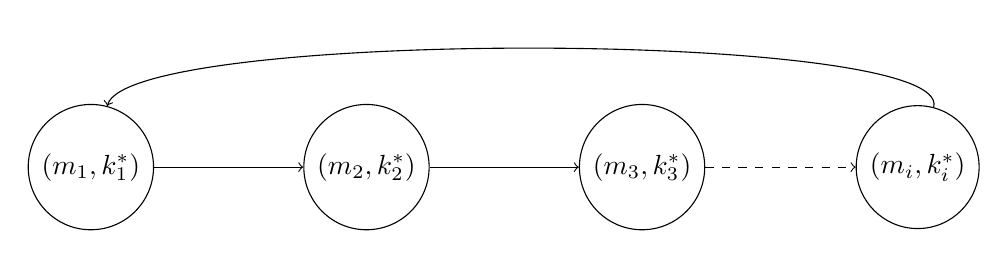
\begin{tikzpicture}[node distance={35mm}, main/.style = {draw, circle},scale=0.5] 
        \node[main] (1) {$( m_1,k^*_1 )$}; 
        \node[main] (2) [right of=1] {$( m_2,k^*_2 )$}; 
        \node[main] (3) [right of=2]{$( m_{3},k^*_{3} ) $}; 
        \node[main] (4) [right of=3]{$( m_i,k^*_i )$}; 
        \draw[->] (4) to [out=75, in=75, looseness=0.25] (1);
        \draw[->] (1) -- (2); 
        \draw[->] (2) -- (3); 
        \draw[dashed ,->] (3) -- (4); 
    \end{tikzpicture} 
    }
    \caption{An $i$-cycle contained in $PG_{G^*}$}
    \label{fig:cycle}
\end{figure}

We can then construct a new matching by reassigning each agent $m_j$ to the arm indicated by the node it points to, i.e., $k^*_{(j\%i) + 1}$, thus creating a new matching $G'$ with a higher total weight. We then show that if no agent is matched with their most preferred arm, there must be a cycle in $PG_{G^*}$, which contradicts the optimality of $G^*$ as established.

If no agent is matched with their most preferred arm, consider an arbitrary agent $m$. We observe that the node $( m, k )$ has at least one outgoing edge. Suppose the node $( m', k' )$ is the any of them $( m, k )$ is pointing to. We also know that $( m', k' )$ must have at least one outgoing edge that does not point back to $( m, k )$; otherwise, $PG_{G^*}$ would contain a 2-cycle, contradicting the optimality of $G^*$. Therefore, $( m', k' )$ must point to another node, $( m'', k'' )$. To avoid forming a cycle, this chain of nodes would need to grow infinitely, which contradicts the assumption that $\mathcal{M}$ is finite. Thus, there must be at least one agent, denoted $m_1$, who is matched with their most preferred arm under $G^*$.

To complete the proof, we then remove $m_1$ from $\mathcal{M}$ and $k_{m_1}^{G^*}$ from $\mathcal{K}$. We apply the same argument to show that there exists an agent $m_2$ who is matched with their most preferred arm after removing $k_{m_1}^{G^*}$, which could have been preferred to $k_{m_2}^{G^*}$ by $m_2$. This implies that $m_2$'s match under $G^*$ is either their most or second most preferred arm. We continue this argument for the remaining agents by induction, thereby completing the proof.

\end{proof}























\section{Auxiliary Lemmas}

\begin{lemma}\label{lemma:scaling_kl}
    For a given $0<p\leq q\leq1 $ as mean of Bernoulli distribution and $n\in \mathbb{R}^+$, the following inequality holds
    \begin{align*}
        \mathrm{kl}\left(\frac{p}{n},\frac{q}{n}\right)\leq \frac{1}{n} \mathrm{kl}\left(p,q\right).
    \end{align*}
\end{lemma}
\begin{proof}
 We first replace both sides of the inequality with the definition of $\mathrm{kl}$ and write it as:
\begin{align}\label{ineq:kl_n}
    \frac{p}{n} \log\left(\frac{p}{q}\right) + \left(1 - \frac{p}{n}\right) \log\left(\frac{1 - \frac{p}{n}}{1 - \frac{q}{n}}\right) \leq \frac{1}{n}\left(p \log\left(\frac{p}{q}\right) + (1 - p) \log\left(\frac{1 - p}{1 - q}\right)\right),
\end{align}

For \eqref{ineq:kl_n} to hold, it suffices to prove:
\begin{align*}
    \left(1 - \frac{p}{n}\right) \log\left(\frac{1 - \frac{p}{n}}{1 - \frac{q}{n}}\right) \leq \frac{1}{n} (1 - p) \log\left(\frac{1 - p}{1 - q}\right),
\end{align*}
which is equivalent to:
\begin{align}\label{ineq:kl_scaling_2}
    \left(\frac{1 - \frac{p}{n}}{1 - \frac{q}{n}}\right)^{n - p} \leq \left(\frac{1 - p}{1 - q}\right)^{1 - p}.
\end{align}

Now we can observe that \(n = 1\) makes both sides of inequality \eqref{ineq:kl_scaling_2} equal. Assuming that \(n \geq 1\), we prove that \(\left(\frac{1 - \frac{p}{n}}{1 - \frac{q}{n}}\right)^{n - p}\) is a decreasing function in \(n\). Then we finish the proof by showing that the derivative of \(\left(\frac{1 - \frac{p}{n}}{1 - \frac{q}{n}}\right)^{n - p}\) with respect to \(n\) is always negative.

After renaming \(v = n - p\) and \(u = \frac{n - p}{n - q}\), we can write:
\[
    \frac{d u^v}{dn} = u^v \left(\frac{dv}{dn} \log u + \frac{v \frac{du}{dn}}{u}\right),
\]

To wrap up the proof, we need to show that this derivative is always negative, which implies \(u^v\) is decreasing in \(n\). For this argument to be correct, the following inequalities should hold:
\begin{align}
    u^v \left(\frac{dv}{dn} \log u + \frac{v \frac{du}{dn}}{u}\right) \leq 0 &\implies \frac{dv}{dn} \log u + \frac{v \frac{du}{dn}}{u} \leq 0, \nonumber\\
    &\implies \log \left(\frac{n - p}{n - q}\right) \leq \frac{q - p}{n - q}, \nonumber\\
    &\implies \left(1 + \frac{q - p}{n - q}\right) \leq e^{\frac{q - p}{n - q}}. \label{ineq:derivation}
\end{align}

By the inequality \(\forall x > 0, \left(1 + x\right)^{\frac{1}{x}} \leq e\), inequality \eqref{ineq:derivation} is always correct. Thus, we proved that \(\left(\frac{1 - \frac{p}{n}}{1 - \frac{q}{n}}\right)^{n - p}\) is decreasing in \(n\), which completes our proof.


\end{proof}

\begin{lemma}\label{lemma:c_whhmab_kl1}
For a given $m_1,m_2 \in \mathcal{M}$,$k_1,k_2\in \mathcal{K}$, and $n,n_1,n_2\in \mathbb{N}^+$ such that $\hat{\mu}_{m_1,k_1}(t) \leq \hat{\mu}_{m_2,k_2}(t)$ and $n_1\leq n_2$, We define $d^n_{m,k}(t)$ as 
    $$d^n_{m, k}(t)\coloneqq\sup \left\{q \geq 0: n\ \mathrm{kl}\left(\hat{\mu}_{m,k}(t), q\right) \leq \log t+4 \log \log t\right\},$$
     the following inequalities hold
    \begin{enumerate}
        \item $d^{n_1}_{m, k}(t) > d^{n_2}_{m, k}(t),$
        \item $d^{n}_{m_1, k_1}(t) \leq d^{n}_{m_2, k_2}(t).$
    \end{enumerate}

\end{lemma}
\begin{proof}
     For the first part, according to the definition, \(d^n_{m,k}\) is decreasing in \(n\). This is because increasing \(n\) requires \(q\) to be closer to \(\hat{\mu}_{m,k}(t)\), as \(\mathrm{kl}(p', q')\) increases with \(q'\). Therefore, since \(n_1 \leq n_2\), we conclude that \(d^{n_1}_{m, k}(t) > d^{n_2}_{m, k}(t)\).

    For the second part we basically use the fact that $d^n_{m,k}(t)\geq \hat{\mu}_{m,k}(t)$. Assuming $q^*=d^n_{m_2,k_2}(t)$, then we know that 
    \begin{align}\label{fct:lemma_kl_1}
        n\mathrm{kl}\left(\hat{\mu}_{m_2,k_2}(t),q^*\right) = \log t + \log\log t,
    \end{align} 
    We then we can prove that $d^n_{m_1,k_1} \leq q^*$. Accordingly we put $q^*$ in definition of $d^n_{m_1,k_1}$ and write
    \begin{align*}
        \hat{\mu}_{m_1,k_1}(t) \leq \hat{\mu}_{m_2,k_2}(t)&\overset{}{\implies} q^*-\hat{\mu}_{m_2,k_2}(t) \leq q^*-\hat{\mu}_{m_1,k_1}(t),\\
        &\overset{(a)}{\implies} \mathrm{kl}\left(\hat{\mu}_{m_2,k_2}(t),q^*\right) \leq \mathrm{kl}\left(\hat{\mu}_{m_1,k_1}(t),q^*\right),\\
        &\overset{(b)}{\implies} n\mathrm{kl}\left(\hat{\mu}_{m_1,k_1}(t),q^*\right) \geq \log t + \log\log t,\\
        &\implies d^n_{m_1,k_1}(t) \leq q^*,\\
        &\implies d^n_{m_1,k_1}(t) \leq d^n_{m_2,k_2}(t) .
    \end{align*}
    while (a) is implied by the fact that $\mathrm{kl}(p',q')$ increases as $\abs{q'-p'}$ grows and (b) is implied by equation \ref{fct:lemma_kl_1}.
\end{proof}
\begin{lemma}\label{lemma:main_c_whh}\todo{check this lemma}
    For a given $n \in \mathbb{N}^+$ and $G$ as a perfect matching between set of agents $\mathcal{M}$ and arms $\mathcal{K}$, We define $d_G(t)$ and $d^n_G(t)$ relatively as 
    $$d_G(t)\coloneqq\sup \left\{q \geq 0: N^{\pi}_G(t)\ \mathrm{kl}\left(U\left(G;\bm{\hat{\mu}}(t)\right), q\right) \leq \log t+4 \log \log t\right\},$$
      $$d^n_G(t)\coloneqq\sup \left\{q \geq 0: n\ \mathrm{kl}\left(U\left(G;\bm{\hat{\mu}}(t)\right), q\right) \leq \log t+4 \log \log t\right\},$$
     Then
    \begin{align*}
        d_G(t) \geq \frac{1}{M}\sum_{\langle m,k \rangle \in G} d_{m,k}(t).
    \end{align*}
\end{lemma}

\begin{proof}
First we define
$$n_{\min} \doteq \min_{\langle m,k \rangle \in G} \abs{\mathcal{N}^\pi_{m,k}},$$
and
$$N \doteq \abs{\mathcal{N}^\pi_G}.$$

Then we can observe that $N \leq n_{\min}$ cause all the edges $\langle m,k \rangle$ could also be observed by each of the $K^{M-1}$ edges. Thus, using the result of Lemma \ref{lemma:c_whhmab_kl1} we can write the LHS as
\begin{align}
    d_G(t) = d^N_G(t) &\geq d^{n_{\min}}_G(t),\nonumber\\
    &= \sup \left\{q \geq 0: n_{\min}\ \mathrm{kl}\left(\hat{U}_{G}(t), q\right) \leq \log t+4 \log \log t\right\},\nonumber\\
    &= \sup \left\{q \geq 0: n_{\min}\ \mathrm{kl}\left(\sum_{\langle m,k \rangle \in G} \hat{\mu}_{m,k}(t), q\right) \leq \log t+4 \log \log t\right\},\nonumber\\
    &\geq \sup \left\{q \geq 0: n_{\min}\ \mathrm{kl}\left(M\prod_{\langle m,k \rangle \in G} \left(\hat{\mu}_{m,k}(t)\right)^{\frac{1}{M}}, q\right) \leq \log t+4 \log \log t\right\},\nonumber\\
    &\geq \sup \left\{\sum_{\langle m,k \rangle \in [G]} q_{m,k} \geq 0: n_{\min}\ \mathrm{kl}\left(\prod_{\langle m,k \rangle \in G} \left(\hat{\mu}_{m,k}(t)\right)^{\frac{1}{M}}, q_{m,k}\right) \leq \log t+4 \log \log t\right\},\nonumber\\
    &\geq \sup \left\{\sum_{\langle m,k \rangle \in [G]} q_{m,k} \geq 0: n_{\min}\ \sum_{\langle m,k \rangle \in G} \mathrm{kl}\left( \frac{\hat{\mu}_{m,k}(t)}{M}, q_{m,k}\right) \leq \log t+4 \log \log t\right\}. \label{lemma:main_lhs}
\end{align}

Now we write the RHS as
\begin{align}
     \sum_{\langle m,k \rangle \in G} d_{m,k}(t) &= \sum_{\langle m,k \rangle \in G} \sup \left\{q \geq 0: \abs{\mathcal{N}^\pi_{m,k}(t)}\ \mathrm{kl}\left(\hat{\mu}_{m,k}(t), q\right) \leq \log t+4 \log \log t\right\},\nonumber\\
     &\leq  \sum_{\langle m,k \rangle \in G} \sup \left\{q \geq 0: n_{\min}\ \mathrm{kl}\left(\hat{\mu}_{m,k}(t), q\right) \leq \log t+4 \log \log t\right\}.\label{lemma:main_rhs}
\end{align}

Now we finish the proof by showing that (\ref{lemma:main_lhs}) $\geq$ (\ref{lemma:main_rhs}). So, we write 
\end{proof}
\begin{lemma}\label{lemma:dtilde}
Lets assume that $\tilde{\mu}_{m,k}(t) = \hat{\mu}_{m,k}(t) + \epsilon$ for a fixed $\epsilon \geq 0$, then $$\tilde{d}_{m,k}(t) > \tilde{\mu}_{m,k}(t) \implies d_{m,k}(t) > \hat{\mu}_{m,k}(t).$$
\end{lemma}
\begin{proof}
We start the proof by arguing that $\tilde{d}_{m,k}(t)-d_{m,k}(t) \leq \epsilon$. Then we can write
\begin{align*}
    \tilde{d}_{m,k}(t) > \tilde{\mu}_{m,k}(t) &\implies \tilde{d}_{m,k}(t) -\epsilon > \tilde{\mu}_{m,k}(t) - \epsilon,\\
    &\implies \tilde{d}_{m,k}(t) -\epsilon > \hat{\mu}_{m,k}(t),\\
    &\implies d_{m,k}(t) > \hat{\mu}_{m,k}(t).
\end{align*}
\end{proof}
































































\end{document}
